%% probabilistic_framework.tex
The introduction in \secref{intro_motivation} describes that preventing early commitment \cite{marr_vision_2010} is considered a fundamental property of the human visual system that is absent in current deep learning frameworks.
The previous chapter introduced neuroscientific findings that could explain why this problem is absent in the human brain and that are considered the principles implementing the findings of the Gestalt psychology \cite{ellis_source_1938, kohler_gestalt_1992, wagemans_century_2012, hamlyn_psychology_2017}.

In the following, a novel framework incorporating these identified principles is proposed.
The focus is on translating the two stages described in \secref{neuroscience_findings} into a computational framework.
Incorporating further stages required for object classification and scene interpretation as described in the long-term vision in \secref{biologial_inspiration_vision} remains an open task for future research.
While the inspiration and principles are based on previous research, a novel computational framework is described in this chapter.

\section{3-Staged Model}\seclbl{framework_3_staged_model}
Some of the neuroscientific principles described in \secref{neuroscience_findings} have been explored in the theory of self-organising projection fibres \sidecite{wiskott_face_1996, wiskott_face_1997, fernandes_self-organization_2015} (c.f. \secref{projection_fibres}). However, these approaches do not yet scale to natural images except for human faces \sidecite{wolfrum_recurrent_2008}. This is because most work in this area has neglected to model the learning and the dynamics of rich sets of net fragments in the visual cortex, which are fundamental according to the theory of natural intelligence \sidecite{von_der_malsburg_theory_2022}.

This section describes a novel system based on binary neurons with the potential to scale to natural images since it extends the projection fibres with net fragments.
The proposed system comprises three main components: A first stage \emph{S0} that extracts features from the image, a stage \emph{S1} that builds an overlay of net fragments, and a stage \emph{S2} that uses projection fibres to map them to object prototypes.
I call the stage \emph{S0} the sensory system, \emph{S1} the feature building stage, and \emph{S2} the prototype stage.
In the context of biology, the sensory stage \emph{S0} could stand for the eyes translating visual information into neuronal activity \sidecite{grill-spector_human_2004}, \emph{S1} could stand for the primary visual cortex \sidecite{tong_primary_2003}, and \emph{S2} for the ventral stream \sidecite{goodale_separate_1992} and an area in the temporal cortex \cite{miyashita_inferior_1993}.
In the following, an overview of these three building blocks is given from a computational perspective, and the advantages of the proposed framework are described.
Afterwards, more implementation details are provided, making the framework more concrete.

\subsection{Building Blocks}\seclbl{framework_building_blocks}
\begin{figure}[h]
    \centering
    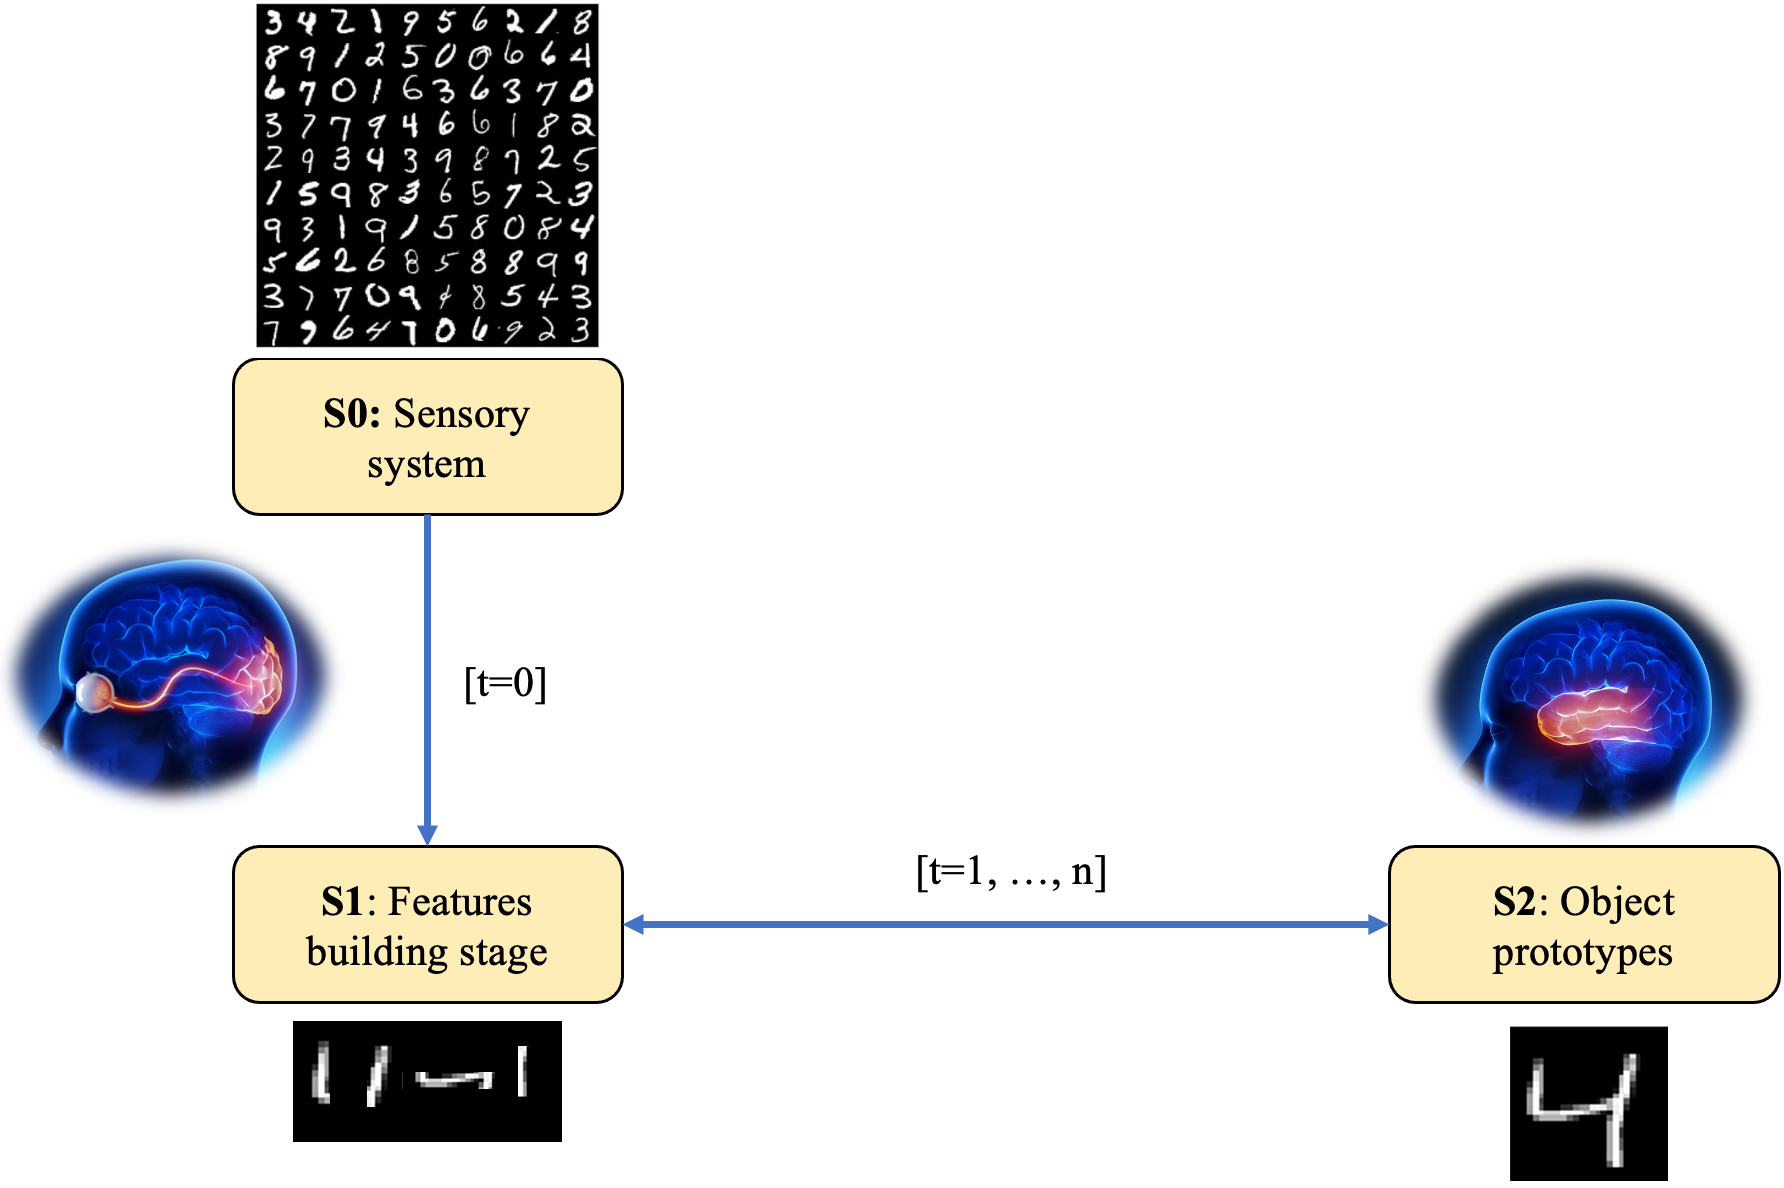
\includegraphics[width=0.99\textwidth]{system overview}
    \caption[Overview of the framework]{Overview of the framework. \emph{S0} extracts features from the image at timestep $t=0$, \emph{S1} builds net fragments, and \emph{S2} maps them to object prototypes using projection fibres. The network refines the features over multiple timesteps in which inhibition is increased, and cells without sufficient support are turned off.}
    \figlbl{system_overview}
\end{figure}

In \figref{system_overview}, an overview of the building blocks of the proposed framework is provided. After the sensory stage extracted features and some initial net fragments have been built in \emph{S1}, an inhibition phase \sidecite{coombs_specific_1955, vogels_inhibitory_2011} lasting multiple timesteps turns off cells that do not receive sufficient lateral support. Furthermore, the project fibres \sidecite{greig_molecular_2013} between \emph{S1} and \emph{S2} run in both directions, not only mapping net fragments to reference frames but also providing feedback to \emph{S1} in the form of additional support for well-known objects.
All these building blocks utilise a binary neuron, which I call the Bernoulli neuron, as its output state is sampled from a Bernoulli distribution.
Utilising Bernoulli neurons lead to sparse and distributed binary network activities, which possess properties that enhance robustness to noise within a network \sidecite{ahmad_properties_2015}.

\paragraph{Sensors System \emph{S0}.} A typical input to the sensory stage is an image having one (grey-scale) or three (RGB) colour channels. Therefore, such an image can be interpreted as having one or three features at every spatial location.
The sensory system extracts multiple features by considering a spatial neighbourhood, thereby increasing the number of features at each location.
For example, a sensory system can be a set of hand-crafted or Gabor filters \sidecite{gabor_theory_1946, granlund_search_1978} applied at all image positions or the first layer of a pre-trained CNN \sidecite{lecun_backpropagation_1989}.

\paragraph{Feature Building Stage \emph{S1}.} The feature building stage is a single layer with lateral connections \sidecite{gilbert_lateral_1990} that builds an overlay of net fragments. Input from the sensory system activates some feature neurons in \emph{S1}. However, their continued firing relies on receiving support from a sufficient number of other activated neurons that are laterally connected to them \sidecite{von_der_malsburg_concerning_2018}. Initially activated neurons that do not receive enough lateral support deactivate after a short period due to inhibition \sidecite{vogels_inhibitory_2011}.

The lateral connections are learned through self-organisation \cite{hebb_organization_1949}. Patterns occurring repeatedly in the training data will constantly activate the same cells simultaneously. Using Hebbian learning \cite{hebb_organization_1949} strengthens the connection between these cells, and the pattern is ``stored'' in a net fragment \cite{von_der_malsburg_concerning_2018}. The inhibition strength increases during training to account for the increasing numbers of lateral connections so that cells with fewer active connections can be suppressed in favour of those with more connections, allowing the latter to acquire even more lateral connections.

Consequently, many neurons might be activated by the sensory stage, but only the ones supporting each other remain active.
Therefore, it is essential to view the process from the perspective that active neurons are integral parts of consistent global net fragments, and only the support from neurons within the same net fragments enables them to persist.

To facilitate various patterns and the coherent networks underlying them, neurons require many excitatory connections. To prevent cross-talk between net fragments (where a neuron receives support from a network it does not belong to), a sustained-firing condition is required in the form of a minimum number of connections that must be activated.

\paragraph{Object Prototype Stage \emph{S2}.} Stage \emph{S2} has the same structure as \emph{S1}. However, it has a smaller coverage area, focusing on object-centred representations rather than encompassing the entire visual field. It allows lateral connections with a greater range \sidecite{stettler_lateral_2002, pessoa_understanding_2014}, essential to represent larger-scale structures like objects. 
Thus, this stage contains isolated net fragments that can be considered object prototypes invariant to translation, scale, and orientation.

In the object recognition process, corresponding net fragments in \emph{S1} are mapped to object prototypes in \emph{S2} through active projection fibres. Here, ``corresponding'' refers to neurons relating to the same point on the object's surface.
The projection fibres between \emph{S1} and \emph{S2} are grouped in maplets, whereby a maplet comprises a collection of fibres that establish one-to-one connections between all neurons in a small patch of \emph{S1} and all neurons in a small patch of \emph{S2} in a topological manner. These topological connections link neighbouring neurons in \emph{S1} to neighbouring neurons in \emph{S2}. Both \emph{S1} and \emph{S2} are divided into overlapping patches, and for each pair of patches - one in \emph{S1} and one in \emph{S2} - a corresponding maplet exists.

Control units initiate activation of a maplet when they observe a high pattern correlation between the signals carried by its fibres from \emph{S1} and the signals on their target neurons in \emph{S2}. They inhibit competing control units: Many projection fibres can initially be activated, but only those activated S2 neurons with sufficient lateral support can remain active.
Consequently, the activated projection achieves a homeomorphism, where neurons of a particular feature type in \emph{S1} are connected to neurons of the same type in \emph{S2} and neurons connected in \emph{S1} activate neurons connected in \emph{S2}.

\begin{comment}
\paragraph{Bernoulli Neuron.} The aforementioned components are implemented using a novel type of neuron I call the Bernoulli neuron (c.f. \secref{bernoulli_neuron}). This neuron interprets the incoming activity as an activation probability and samples a binary signal from a Bernoulli distribution based on this probability. Utilising Bernoulli neurons lead to sparse and distributed binary network activities, which possess properties that enhance robustness to noise within a network \sidecite{ahmad_properties_2015}.

Bernoulli neurons allow the modelling of net fragments with lateral support. Preliminary experiments have indicated that using non-binary artificial neurons is not well suited for learning net fragments. For instance, dealing with weak or strong positive activations poses challenges when employing Hebbian updates. In contrast, the Bernoulli neuron tends to turn off negative or very weak activations, while strong activations tend to become $1$. This behaviour prevents the establishment of connections between weakly activated neurons. Furthermore, sampling from a Bernoulli distribution introduces a small amount of randomness to the network, encouraging parallel paths and increasing robustness (c.f. \secref{bernoulli_neuron}). This is especially important to train lateral connections of alternative cells (c.f. \secref{framework_alt_cells}).

\subsection{Theory of Natural Intelligence}
The proposed architecture is based on a correspondence-based system \sidecite{zhu_maplets_2004} that achieves invariance by routing signals through rapidly changing connections \sidecite{wiskott_face_1996, olshausen_neurobiological_1993, arathorn_map-seeking_2002}.
Based on the neuroscientific findings summarised in \secref{neuroscience_findings_correspondence_finding}, I argue that the mapping between input data and stored object prototypes, as outlined in the previous sections, is closely related to the human brain's functionality and in line with findings from neuroscience \sidecite{vogels_inhibitory_2011, kandel_principles_2013, olshausen_emergence_1996, payeur_burst-dependent_2021} and psychology \sidecite{ellis_source_1938, kohler_gestalt_1992, wagemans_century_2012, hamlyn_psychology_2017}.

This argumentation is backed by the theory of natural intelligence \cite{von_der_malsburg_theory_2022}.
As this theory serves as inspiration for this thesis, the relationship between their theoretical concepts and the proposed framework is discussed in the following.
The theory of natural intelligence describes how the brain develops an overlay of net fragments (c.f. \secref{natural_intelligence}) consisting of neurons supporting each other to remain active.
This behaviour is implemented in the feature building stage \emph{S1}: The sensory signal from \emph{S0} activates many neurons from which only the ones receiving enough lateral support remain active. Furthermore, it is implemented in the control units of the maplets. Initially, many maplets can be active, allowing various active fibres between \emph{S1} and \emph{S2}. However, an inhibitory signal serves as competition between these maplets, allowing only the most consistent to remain active after a short transient phase.

The theory also describes that an object is represented by multiple net fragments, whereby each net fragment represents a part of the surface of that object.
As described above, an object is represented in \emph{S1} and \emph{S2} as an overlay of net fragments. Furthermore, projection fibres map net fragments formed in \emph{S1} to object prototypes in \emph{S2}.
Thus, a hierarchy of attractor networks represents an object, as suggested in the theory of natural intelligence.

Furthermore, it is postulated in the theory that self-organisation is the key algorithm to form such fragments and the learning mechanism loops between activity and connectivity for a short time until an attractor state is reached.
In the context of this work, self-organisation is used to organise lateral connections and projection fibres. In fact, local Hebbian learning \cite{hebb_organization_1949} is applied to learn the support strength between neurons, allowing the network to turn off neurons that are not part of the dominating net fragments.
Furthermore, Hebbian plasticity initiates the mapping process by triggering control units \cite{anderson_shifter_1987}.
Looping between activity and connectivity is implemented with projection fibres. 
Each prototype in \emph{S2} is considered a hypothesis of what object is present in the input. A net fragment in \emph{S1} can be mapped to multiple prototypes, and each active fragment supports specific hypotheses in \emph{S2}. The hypotheses act back on \emph{S1} and support its fragments. Thus, the activity part is realised by \emph{S1} when supporting or turning off cells and the connectivity part is realised by projection fibres mapping the net fragments to \emph{S2}, thereby providing feedback to \emph{S1}.

Overall, I argue that the proposed framework is an implementation following strictly the theory of natural intelligence \sidecite{von_der_malsburg_theory_2022}. Thus, according to leading experts in the field, this framework has the ability to make a step towards natural intelligence and emergence. 
\end{comment}

\subsection{Advantages}\seclbl{framework_advantages}
The proposed framework not only prevents early commitment \sidecite{marr_vision_2010} but is expected to have various additional advantages compared to the typical deep learning framework. These are described in the following.

\paragraph{Ambiguity.} The proposed framework permits the persistence of multiple net fragments, enabling the system to handle ambiguity effectively. For example, when presented with a face comprising distinct objects (c.f. \figref{sdp_mountain}), both the net fragments responsible for abstract faces and those associated with individual objects become concurrently active. Consequently, the model can simultaneously attend to these net fragments, utilising attention in its original sense rather than the conventional deep neural network (DNN) interpretation \sidecite{niu_review_2021}. I speculate that this represents a fundamental distinction from neural networks that are typically compelled to represent the entire scene within a single high-dimensional dense vector.

\paragraph{Robustness.} An input of a neural network is usually represented with a floating-point vector which is sequentially processed by mathematical functions (e.g. with neural layers). Artificial networks, in particular, are not robust to noise and are susceptible to adversarial attacks \sidecite{akhtar_threat_2018}. A binary vector, on the other hand, has different mathematical properties and is more robust against noise and adversarial attacks, especially if they are sparse and distributed\sidenote{Only a small portion of the bits are ``on'', and representations differ by multiple binary bits.} \sidecite{ahmad_properties_2015}.
Subsampled or noisy vectors are still semantically similar and are close to the original vectors when compared, for example, by counting the overlap of bits between two vectors.
Furthermore, the model builds consistency at every point in the network, making it more robust than when consistency is built at a single point \sidecite{wagner_robustness_2013}.

\paragraph{Object-Independent Transformations.} The same projection fibres are applied to all object prototypes, allowing the model to learn object-independent transformations. For example, an object might be slightly stretched, rotated, or deformed compared to the stored prototypes. The projection fibres learn to ignore slight deformations independent of the object type. This allows the architecture to learn transformation invariance and to transfer this capability to new objects that have not been transformed in the training data.
Furthermore, it allows adding objects dynamically to static reference frames, implementing lifelong learning \sidecite{parisi_continual_2019} without the risk of catastrophic forgetting \sidecite{kirkpatrick_overcoming_2017, liu_overcoming_2021}.

\section{Bernoulli Neuron}\seclbl{bernoulli_neuron}
The previous section provided an overview of the proposed framework's inspiration, building blocks, and advantages. In the following, the building blocks are described in more detail, starting with the Bernoulli neuron.
In traditional neural networks, neurons exhibit dense activity, meaning that even when applying the rectified linear unit (ReLU) activation function (c.f. \eqref{act_functions}), many neurons remain active (above zero) \sidecite{rhu_compressing_2018}. However, biological neurons have different characteristics than artificial neural networks \sidecite{kandel_principles_2013}.

Preliminary experiments have indicated that using non-binary artificial neurons is not well suited for learning net fragments. For instance, dealing with weak or strong positive activations poses challenges when employing Hebbian updates.
This suggests that implementing net fragments \sidecite{von_der_malsburg_concerning_2018}, similar to the human brain, requires using different principles than the ones used in classical neural networks. Inspired by neuroscientific findings, a probabilistic neuron that samples its activation from a Bernoulli distribution is introduced.
Such a neuron is a binary neuron that does not fire when a certain threshold is reached but uses its internal state as a firing probability. A probabilistic neuron $a_i$ in the context of net fragments is modelled as a probability density function of the form:
\begin{equation}
    p = P(a_i = \text{active} | \text{activity of neighborhood}, \text{environment}) 
\end{equation}

Thus, the probability of a neuron being active depends on the activity pattern of the neurons in its local neighbourhood and factors of the environment (e.g., inhibition or presence of neurotransmitters).
Such a neuron can be implemented using a Bernoulli distribution, i.e., $B(p) = P(X = 1) = p = 1 - P(X=0)$. Having a neuron whose firing probability $p$ is governed by the neighbourhood activity and the environment allows the implementation of the behaviour of net fragments \sidecite{von_der_malsburg_theory_2022, von_der_malsburg_concerning_2018}: After receiving an input, the neurons get excited and fire with a higher probability. However, their firing probability decreases quickly if not supported by neighbouring neurons. Thus, uncertainty and potential net fragments govern timestep 0, while the network reaches an attractor state shortly after. 

\subsection{Properties}
The proposed neuron implements a stochastic process that allows it to fire even when the probability of it firing is low or, conversely, not to fire when the probability is high.
I call this property ``flipping''.
Flipping neurons lead to noise in the network's activations.
However, this noise can be considered a normalisation mechanism within the network, similar to dropout layers \sidecite{hinton_improving_2012}.
The presence of neurons that can flip encourages the network to learn multiple parallel paths and to ignore the noise in its activations.
Furthermore, using many binary neurons and sparse network activations increases the robustness of the network \sidecite{ahmad_properties_2015}.
During inference, the stochastic process can be disabled using a fixed threshold of $0.5$, resulting in a more stable network.

Moreover, flipping neurons help to implement alternative pathways and cells required when a single cell is part of two mutually exclusive net fragments \sidecite{von_der_malsburg_neural_1987}.
Alternative cells are a set of cells with afferent connections. The stochastic property of Bernoulli neurons helps to solve the symmetry problem by encouraging each cell to undergo divergent connectivity changes during training so that it becomes part of mutually exclusive net fragments.

\subsection{Practical Considerations}
To prevent the network from being dominated by noise, it is crucial that most of the activation probabilities do not cluster around a mean value of $\mu = 0.5$. Otherwise, a significant proportion of neurons would have high uncertainty about whether they should fire, leading to random firing patterns. This uncertainty problem occurs mainly in the initial phase of training when the network is not yet trained and therefore dominated by uncertainty.

This issue can be mitigated by pushing the activation probabilities towards $0$ or $1$. A simple approach is to apply the softmax function or to adjust the activation probabilities by a power factor $s$, i.e. $\boldsymbol{a} := \boldsymbol{a}^s$. The softmax function shifts the probabilities uniformly towards $0$ or $1$ while using a large factor $s$ drives most activations predominantly towards $0$, and only high probabilities can remain high.

The advantage of using a factor $s$ is its adaptability: It can be set to a high value in the initial training phase and gradually lowered towards one as training progresses. This allows scoping with the network's uncertainty that reduces during training.


\section{Processing Loops}\seclbl{model_overview}
The network requires different kinds of data processing loops that are divided as follows:
The slow loop iterates through the images in the dataset; the medium loop iterates through different views of an image; and during the fast loop, inhibition takes place over multiple steps, whereby neurons that do not receive enough support are turned off.
At each timestep, the innermost loop executes a step. Once the innermost loop is completed, a step is executed in an outer loop, and the process repeats. The specifics of these loops are described in the following.

\begin{figure}[h]
    \centering
    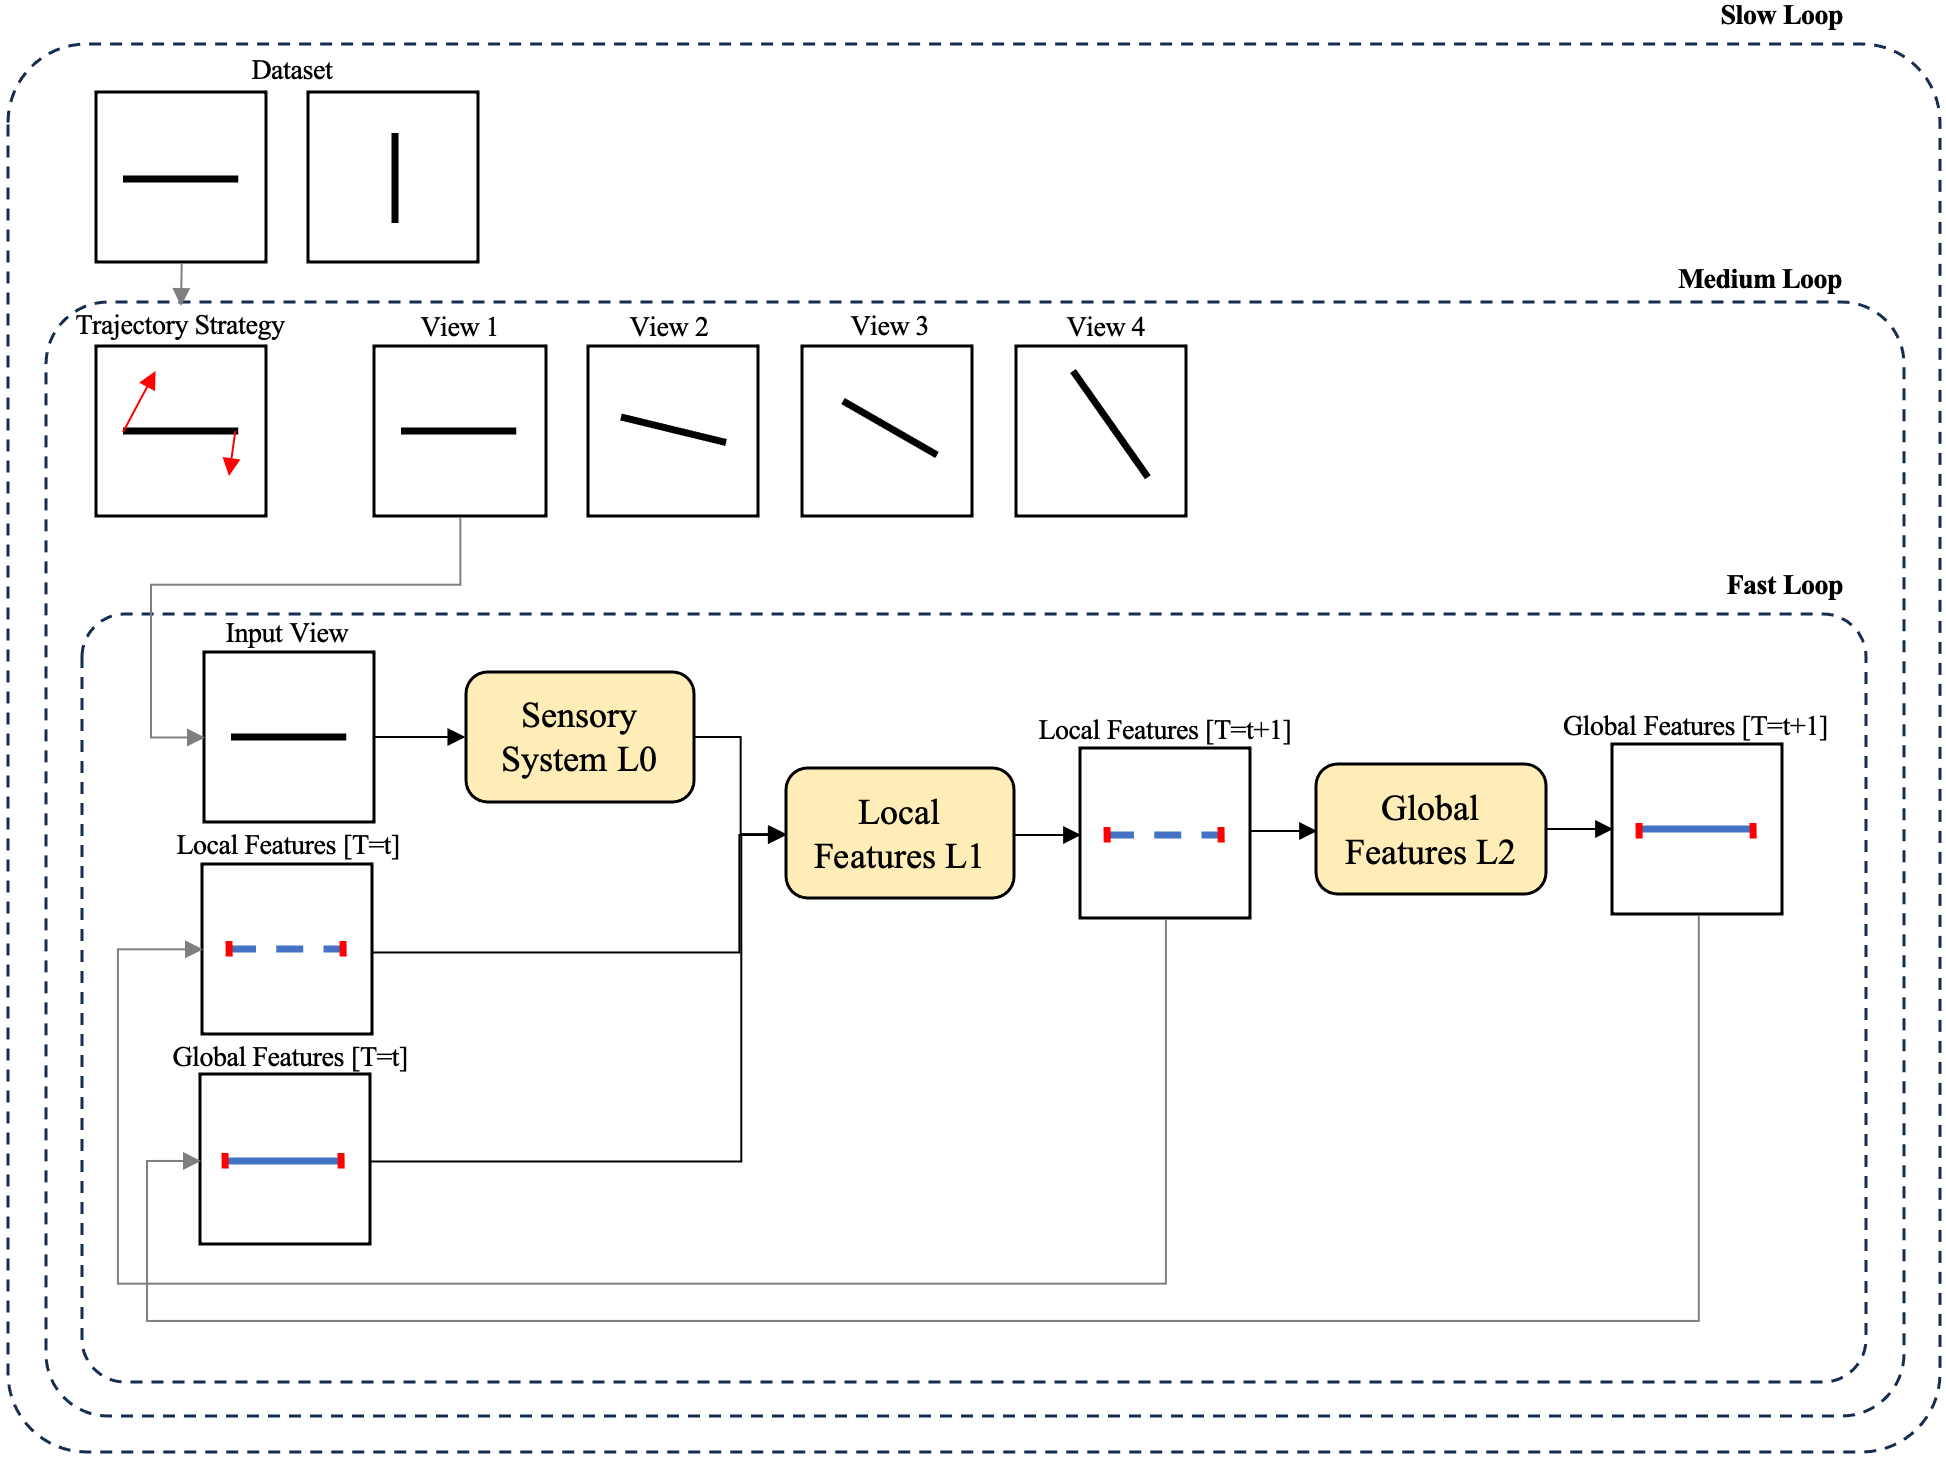
\includegraphics[width=0.99\textwidth]{lateral_loops.png}
    \caption[Processing loops of the network]{Processing loops of the network. From each sample in the dataset (slow loop), multiple views are generated (medium loop), and each view is processed over multiple timesteps by the model (fast loop).}
    \figlbl{lateral_loops}
\end{figure}

\paragraph{Slow Loop.} The dataset comprises multiple images. Each image in the dataset is processed one after the other, building the outermost loop. In \figref{lateral_loops}, an outer loop with a dataset containing vertical and horizontal lines is depicted, similar to data used in the conducted experiments (c.f. \secref{exp_dataset}). However, depending on the application, different datasets could be used.

\paragraph{Medium Loop.} For each image in the dataset, different views are sampled using data augmentation. In the experiments conducted in this thesis (c.f. \secref{exp_dataset}), a trajectory strategy is implemented that moves the line continuously from an initial position to a target position.
However, continuous movement is not mandatory, and random data augmentation can also be applied. It is important to inform the network that the same object with an identical inner structure is shown multiple times during the median loop so that it can learn to map it to the same object prototype despite different transformations and viewpoints.

\paragraph{Fast Loop.} From each view, the sensory system creates neural activity that the network processes for $T \geq 1$ timesteps. During these timesteps, inhibition increases, and active cells that do not get lateral support from other cells are turned off. 
The fast loop aims to iteratively improve the net fragments in \emph{S1} and the corresponding object prototypes over time. Therefore, the previous net fragments and object prototypes are fed into \emph{S1} at every timestep, together with the sensory signal.


\section{Sensory System \emph{S0}}\seclbl{framework_s0}
The goal of the sensory system is to perceive an input and extract multiple different features based on spatial neighbourhoods that can be used to build net fragments \sidecite{von_der_malsburg_theory_2022, von_der_malsburg_concerning_2018} in the next stage.
The input shape is $[C_{\text{in}} \times W \times H]$ where $C_{\text{in}}$ is the number of input channels, $W$ the image width and $H$ the image height.
The output of this stage is of shape $[C_{\text{sensor}} \times W \times H]$, where $C_{\text{sensor}}$ is the number of output channels. Typically, $C_{\text{sensor}}$ is much larger than $C_{\text{in}}$, i.e. $C_{\text{sensor}} \gg C_{\text{in}}$.
Each output channel represents a feature. Thus, the sensory system extracts multiple features based on a local neighbourhood at each pixel location.

As described in \secref{framework_building_blocks}, a sensory system can be implemented with hand-crafted filters, Gabor filters \cite{gabor_theory_1946, granlund_search_1978}, or by training a convolutional network \sidecite{lecun_backpropagation_1989} in an autoencoding setting \sidecite{rumelhart_learning_1986}. The advantage of using learned filters over fixed Gabor filters is that they can be optimised for the source data. However, this comes with the cost of additional filter training.

A difficulty is that filter outputs are typically in continuous space and must be converted into a binary activation potential.
One option is to normalise the sensor signal in the range $(0, .., 1)$ and to use this value as a probability to sample from a Bernoulli distribution, similar to the proposed Bernoulli neurons (c.f. \secref{bernoulli_neuron}).
Another approach is to set all activations above a pre-defined threshold to $1$ and to assign 0 to the values below the threshold.
Alternatively, a third option is to use quantisation networks such as VQ-VAEs \sidecite{van_den_oord_neural_2017} as feature extractors. Such networks can map local features to a discrete value that can be translated into a binary activation pattern.


\section{Feature Extracting Stage \emph{S1}}\seclbl{framework_s1}
The objective of \emph{S1} is to build net fragments based on three types of input: The sensory signal, net fragments from the previous timestep, and feedback from the object prototype stage.
These three types of input serve the following purposes:
\begin{itemize}
    \item \textbf{Sensory signal}: The sensory system extracts features from the image to provide initial cell activations. Theoretically, the sensory signal could be used only once at timestep $t=0$. However, feeding the sensory signal into the network at every timestep stabilises the net fragments \sidenote{This can be likened to closing our eyes: After they are closed, we can estimate the location of all objects but with uncertainty. Thus, the net fragments in our brain become unstable, and we can only estimate the object's position based on memories and previous net fragments.}.
    \item \textbf{Previous net fragments}: Net fragments are the output of the stage \emph{S1}, improved over multiple timesteps.
    To access information from the previous timestep, a recurrent connection is required. This connection is implemented by reusing the previous output (previous net fragments) as input.
    \item \textbf{Object prototypes}: The net fragments are mapped to object prototypes in \emph{S2} using maplets. An inverse function is employed afterwards to map the object prototypes back to local features to provide information about detected objects to \emph{S1}.
\end{itemize}

There exist various ways of combining these three types of input signals. For example, the three arrays can be stacked\sidenote{Stacking arrays refers to the process of combining multiple arrays along a specified axis to create a new multidimensional array, e.g. create an array of size $2 \times 2$ out of two arrays with size $1 \times 2$.} to hold all arrays available.
However, stacking all three arrays would lead to a very high-dimensional input.
A more sophisticated approach is to aggregate (some of) the matrices.
In the experiments conducted in this thesis (c.f. \secref{exp_s1}), a straightforward approach is used: The previous net fragments can be overridden by the feedback from the object prototypes if the feedback is plausible.
Only one of these two arrays is used, as these arrays are typically very similar and provide redundant information. The mapping from fragments to object prototypes and back reduces noise, as the feedback of \emph{S2} is not a reconstructed version of the input but rather a reconstruction of an optimised object prototype. Consequently, the feedback of \emph{S2} is typically less noisy and, therefore, preferred.

Nevertheless, the feedback from \emph{S2} is not always correct and, therefore, only incorporated if it is highly similar to the net fragments formed in \emph{S1}. Especially at the beginning of training or when observing unknown objects, the feedback of \emph{S2} should not be incorporated as it can be wrong.
Such invalid feedback can be detected by measuring the similarity between net fragments and feedback, for example, using Jaccard similarity (c.f. \eqref{jaccard}). Thus, the net fragments are only overridden if the error is below a pre-defined threshold and overriding most likely improves results.

\begin{figure}[h]
    \centering
    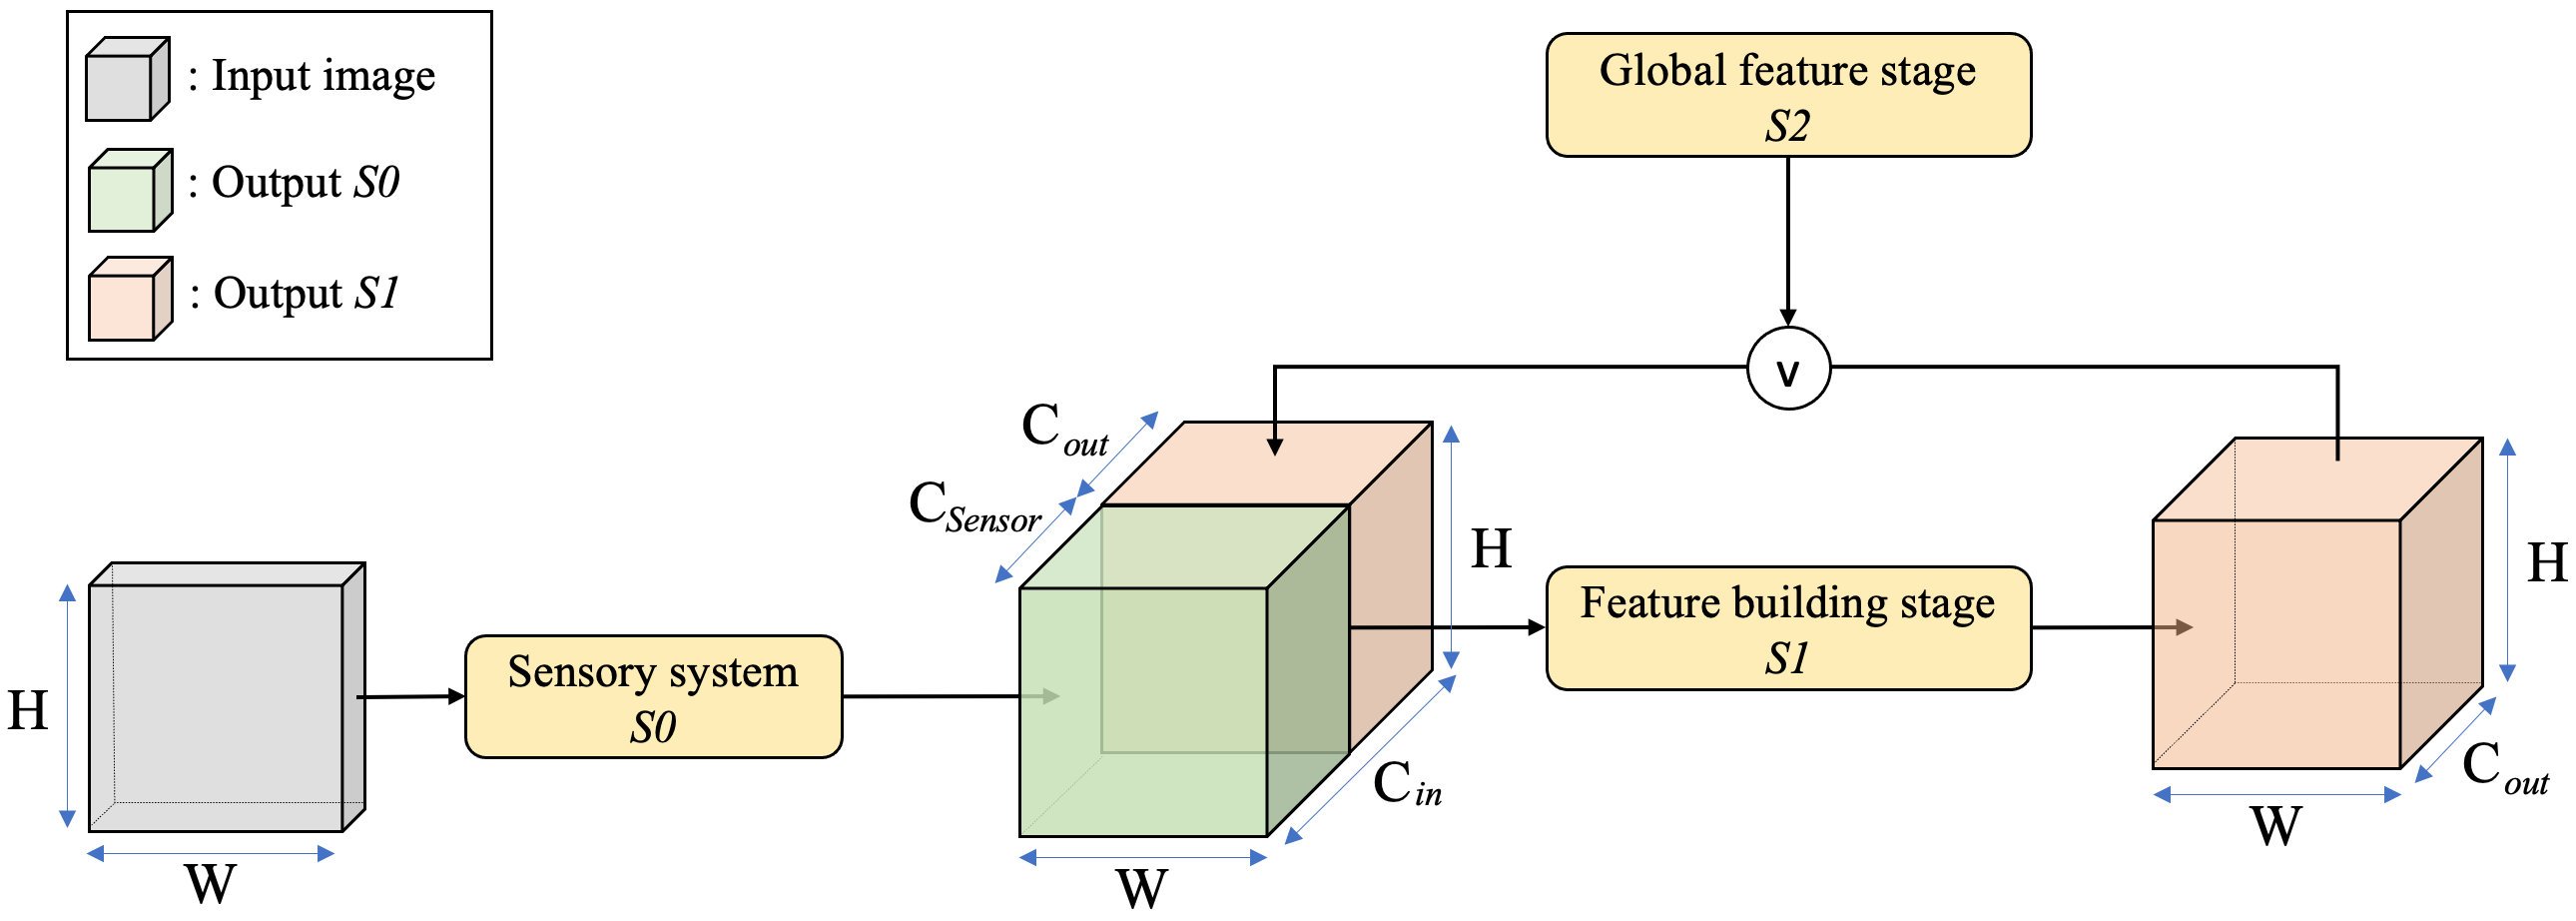
\includegraphics[width=0.99\textwidth]{s1_input}
    \caption[Input and output of \emph{S1}]{Visualisation of the input and output arrays of \emph{S1}. The input into \emph{S1} is the output of the sensory system and the previous output (recurrent connection). The feedback form \emph{S2} can override the previous output.}
    \figlbl{s1_input}
\end{figure}


In the following, the number of input channels is denoted as $C_{\text{in}}$ and the number of output channels is denoted as $C_{\text{out}}$.
Note that the feedback matrix from \emph{S2} has the same shape as the net fragments formed in \emph{S1}.
Since the previous net fragments or the feedback from \emph{S2} is combined with the sensory signal and used as input, the number of input channels is larger than the number of output channels and defined as $C_{\text{in}} = C_{\text{sensor}} + C_{\text{out}}$.
An overview about the input and output of \emph{S1} is depicted in \figref{s1_input}:
The output of \emph{S1} is optionally replaced by the feedback of \emph{S2}. In both cases, this array has a size of $[C_{\text{out}} \times W \times H]$ and is stacked with the output from the sensory system of size $[C_{\text{Sensor}} \times W \times H]$, resulting in an input of size $[C_{\text{in}} \times W \times H]$.


\subsection{Lateral Support}\seclbl{framework_s1_lat_support}
\begin{figure}[h]
    \centering
    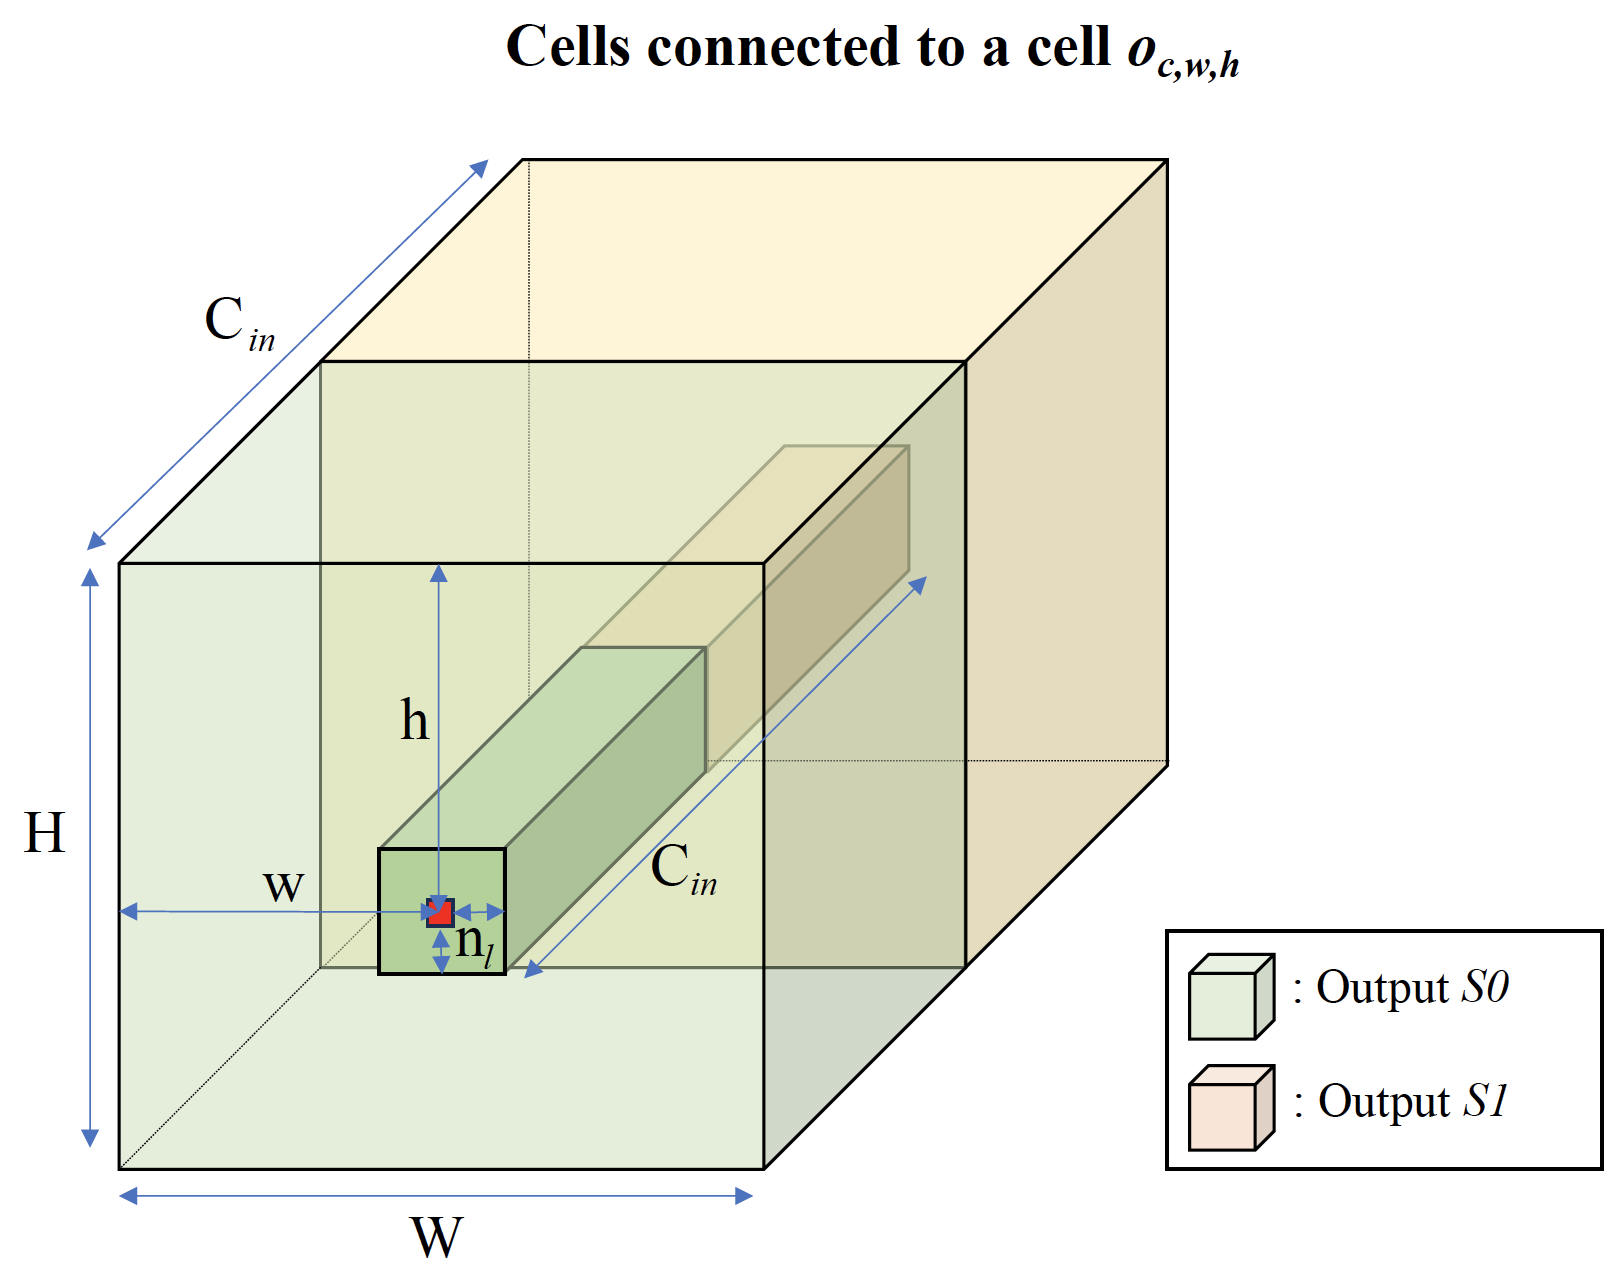
\includegraphics[width=0.89\textwidth]{connected_local-neighbourhood}
    \caption[The local neighbourhood of a cell $o_{c,w,h}$]{The local neighbourhood of a cell $o_{c,w,h}$: The outer cuboid represents the entire input, the inner cuboid the source cells that are connected to the target cell $o_{c,w,h}$.}
    \figlbl{connected_local-neighbourhood}
\end{figure}
%
In this section, it is described how lateral support can be implemented.
A single output cell in \emph{S1} is denoted as $o_{c,w,h}$, where $c \in \{0, ..., C_{\text{out}}\}$ is the output feature channel, and $w \in \{0, ..., W\}$ and $h \in \{0, ..., H\}$ denote the spatial location of the cell.

The lateral connections are limited to a distance of $n_{l}$ cells along the vertical and horizontal axes but are not limited along the input feature channels.
Therefore, an output cell $o_{c,w,h}$ has lateral connections to all inputs within the range $\left[(0, ..., C_{\text{in}}) \times (w - n_l, ..., w+n_l) \times (h - n_l, ..., h+n_l)\right]$.
Such a local neighbourhood is depicted in \figref{connected_local-neighbourhood} for a cell $o_{c,w,h}$.
An input channel contains either features extracted by the sensory system or the previous net fragments. Thus, a cell can access all features detected by the sensory system or the previous cell states (recurrent connection) in its spatial neighbourhood.
Furthermore, according to this definition, the cell is also connected to its own previous cell state at $t-1$.
This type of connection is called self-support and allows a cell to remain active over time by supporting itself.
Self-support is crucial to ensure the network is stable at the beginning of training (c.f. \secref{lateral_init}). However, after training for a short time, lateral connections are built, the inhibition strength increases so that self-support is not sufficient anymore, and lateral support from other cells is required to remain active.

Patterns can appear at different locations within an image, and the network should be able to recognise it independent of its spatial location \sidecite{fukushima_neocognitron_1980, waibel_phoneme_1987}. 
Therefore, lateral support must be position equivariant.
Convolutional architectures solve this problem with convolutional filters shifting over each pixel location \sidecite{lecun_backpropagation_1989}. This mechanism can also be used to implement the lateral connections: When using a convolutional kernel $\boldsymbol{W}$ with size $\left[C_{\text{out}} \times C_{\text{in}} \times (2n_l+1) \times (2n_l+1) \right]$, each output cell has a connection to its local neighbourhood as defined above.
Since this kernel is applied at all cell positions, a cell is supported by neighbouring cells that represent the same pattern regardless of the spatial position.
The weights within a kernel correspond to the support strength, indicating how much a neighbouring cell supports another cell. The support strength of a cell $o_{c,w,h}$ (i.e. how much support a cell receives from its neighbours) can be calculated with the convolutional operation: 
%
\begin{align}\eqlbl{convlat_1}
	o_{c,w,h} = \sum_{c'=0}^{C_{\text{in}}} \sum_{w_i=0}^{2n+1} \sum_{h_i=0}^{2n+1} \boldsymbol{W}_{c, c',w_i,h_i} \cdot o_{c',w-n+w_i,h-n+h_i}
\end{align}
%
Thus, the same weight $\boldsymbol{W}$ is applied at all input locations, defining the support strength of a cell based on its neighbourhood and independent of its position.
This operation corresponds precisely to the output of a convolutional layer without bias term.
Please note that the target cell represents a cell's state at time $t$ (denoted by $c \in \{0, ..., C_{\text{out}}\}$) and can access the state of all source cells (denoted by $c' \in \{0, ..., C_{\text{in}}\}$), i.e. all sensory cells or recurrently connected cell states at $t-1$.

\subsection{Hebbian Updates}\seclbl{framework_hebb_updates}
The previous section introduces how a convolutional kernel $\boldsymbol{W}$ can be used to model the lateral support of neighbouring cells.
In this section, it is described how the support strength, i.e. the weights of $\boldsymbol{W}$, can be learned.
The human brain's learning algorithm is based on local self-organisation and unsupervised (or self-supervised) learning \sidecite{von_der_malsburg_theory_2022}. The biologically most plausible learning algorithm is Hebbian learning \sidecite{hebb_organization_1949}.

Hebbian learning evaluates consistency at each synapse and is well suited for learning lateral connections: If two cells are active together (``fire together''), their weight increases (``wire together'') - this plasticity principle corresponds to the definition of lateral support. During training, the cells are activated in a specific pattern based on the sensory input. Hebbian learning strengthens the connections between simultaneously active cells. Thus, the connection strength between cells associated with the same net fragment is increased, leading to stronger mutual support. Additionally, using negative Hebbian learning, the strength of the lateral support can be reduced between cells that fire in disparity (one of the cells is firing while the other is not).

Hebbian learning is introduced in \secref{hebbian}, and it is described how the weight between two cells changes if they fire together (c.f. \eqref{hebb_1}).
However, lateral support is implemented as a convolutional kernel that is applied at all input positions.
Since the same weight is applied at different positions, the update of a connection depends not only on two cells but on multiple cells:
%
\begin{align}\eqlbl{hebbu_1}
	\Delta w_{c, c',k_w,k_h} = \eta \sum_{w = 0}^{W - 2n_l - 1} \sum_{h = 0}^{H - 2n_l - 1} o_{c,w+k_w,h+k_h} \cdot o_{c',w+k_w,h+k_h}
\end{align}
%
In this formula, $\eta$ is the learning rate, and $k_w \in \{0, ..., 2n_l+1\}$ and $k_h\in \{0, ..., 2n_l+1 \}$ is the kernel index along the horizontal and vertical axis\sidenote{For example, $w_{1, 2,3,4}$ represents the weight between the first output channel and the second input channel, located in the kernel's third column and fourth row.}.
Please note that the weight between two laterally connected cells is increased if both are active simultaneously, whereby one cell is considered as the source cell (denoted as input channel $c'$) of the target cell (denoted as output channel $c$).

During training, the network may encounter similar patterns multiple times, leading to strong connections between specific cells. Therefore, weight must be normalised so that these lateral connection strengths and the post-synaptic activity cannot grow towards infinite. After calculating the weight update and adding it to the weight matrix $\boldsymbol{W}$, the weights are normalised per output channel by dividing each channel by its Euclidean norm. This ensures that the weights are roughly in the range $(0, ..., +1)$.
Therefore, one cell can only provide limited support to another cell, and multiple cells must support a cell to remain active.


%\subsubsection{Breaking the Symmetry} 
%Oja \cite{oja_simplified_1982} stated that all connections within a network trained with Hebbian learning tend to undergo the same updates and that an additional element is required to differentiate the connections. Otherwise, all weights could become similar, and all feature channels depict the same features.

%In practice, this additional element is typically implemented as a type of competition between the feature channels, such as a winner-take-all competition. With winner-take-all, only the neuron with the highest activation is selected for learning. In the case of our network with lateral connections, this means that at each pixel location, precisely one of the feature channels $C$ is updated. However, this is not desirable as it enforces updates even when no features are detected, leading to increased support between neurons that are not even active.

%It was found that this issue can also be resolved if the probabilistic neuron is used and the network is initialised as described in \secref{lateral_init}. When using the probabilistic neuron, neurons are activated with e certain probability. Thus, neurons with a low probability tend not to fire, turning active neurons off. 
%Furthermore, a proper initialisation based on self-support instead of random weights can encourage distinct feature channels.
%This measures differentiation between connection updates, making a competition strategy superfluous.

\subsection{Initialisation}\seclbl{lateral_init}
\begin{figure}[h]
    \centering
    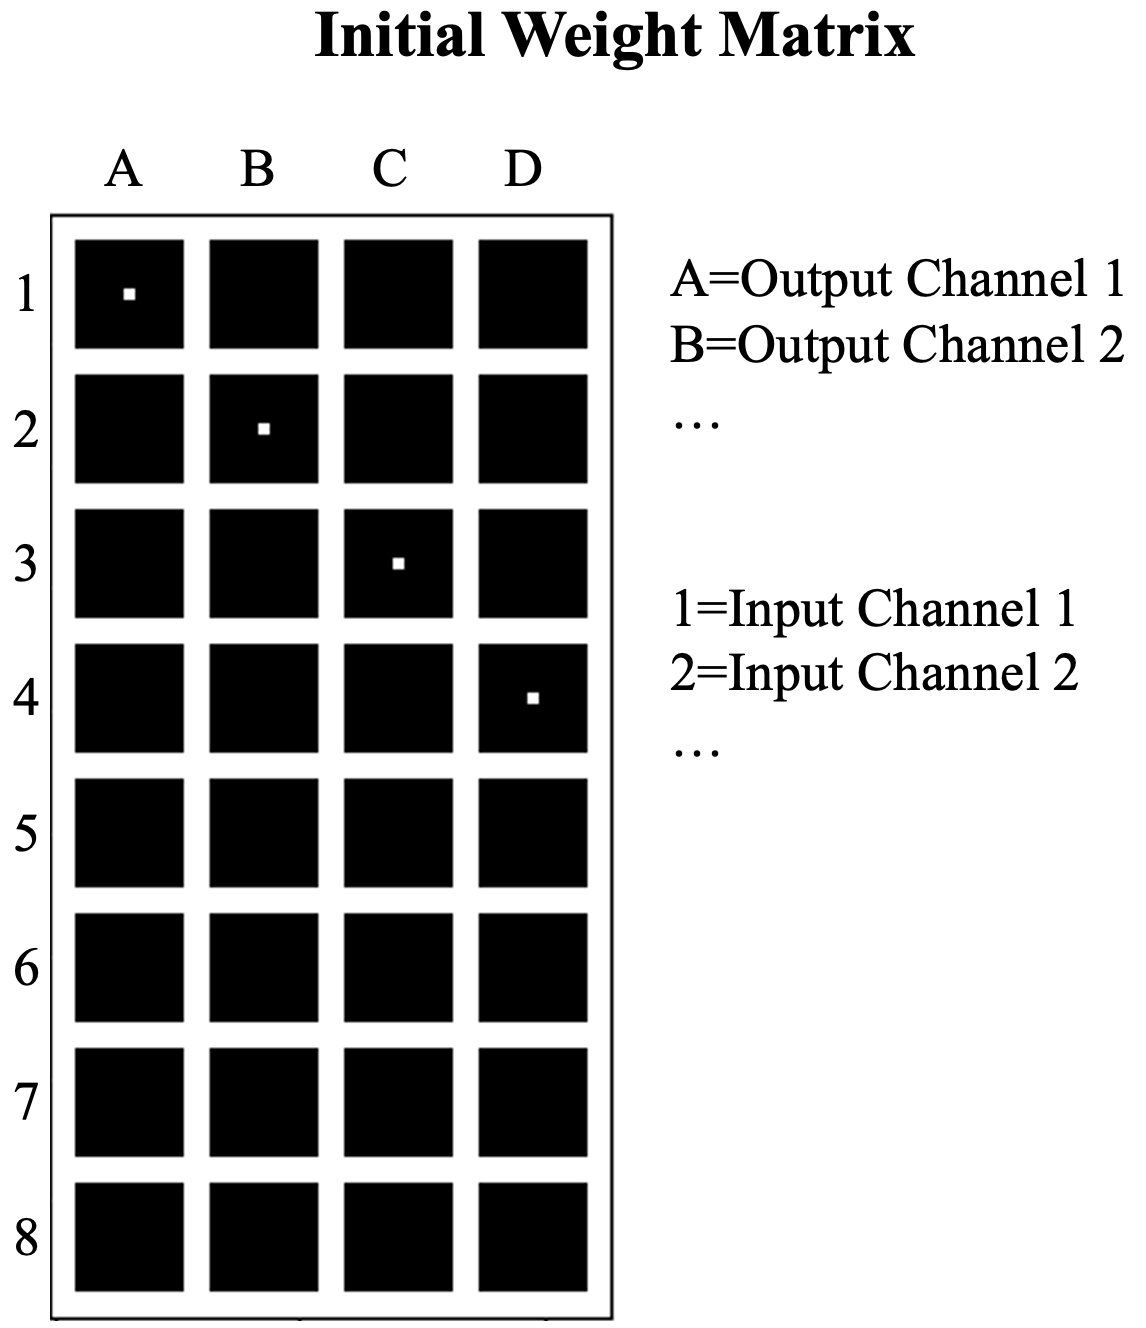
\includegraphics[width=0.6\textwidth]{lateral_init_weights.png}
    \caption[Initialisation of the lateral weight matrix]{Initialisation of the lateral weight matrix. The weight at the middle of a kernel, whose input and output channel have the same index, is set to $1$.}
    \figlbl{lateral_init_weights}
\end{figure}
The previous sections explain that lateral support can be implemented with convolutional kernels and that the weights are learned using the Hebbian rule.
In this section, it is discussed how these kernels should be initialised.
If the kernels are not properly initialised, the activations are unstable and typically converge to weights that activate all or no cells.
A proper initialisation should fulfil the following criteria:

\begin{itemize}
    \item \textbf{Diversity:} A proper initialisation should break the symmetry. If, for example, all kernels are initialised identically, each kernel learns the identical pattern when applying Hebbian updates. This makes all output channels identical, and effectively the model learns only one feature.
    \item \textbf{Stability:} The Hebbian update is calculated after a timestep of the inner loop; therefore, the cells must be stable over timesteps. For example, if the lateral support is only initialised with $0$ values, all cells turn off immediately. In that case, no cell is active after the first timestep, and no support can be learned.
\end{itemize}

An initialisation strategy that fulfils these criteria is when the weights are initialised with self-support.
Self-support means that each cell supports itself to remain active over time, i.e. the recurrent connection to the same cell at the previous timestep must be set to $1$.
Self-support can be implemented by setting all weights $w_{c \times c' \times w \times h}$ of a kernel to $1$ at the indexes that fulfil 
$c' = c$, $w = n+1$, and $h = n+1$. Thus, the weight at the middle of a kernel with the same input and output channel index is set to $1$ while the other weights are set to $0$. This initialisation strategy also works for kernels with a different number of input and output channels and is shown in \figref{lateral_init_weights}.
Such a weight matrix copies the input activations to the output and ensures that the cell's activations at time $t$ and $t+1$ are identical. Therefore, initially, active cells receive a support of $1$ (i.e. one other cell with a lateral weight of $1$ is active).
However, after applying the Hebbian learning rule, the weights are updated to capture the data's statistics so that active cells receive more support.

\subsection{Inhibition}\seclbl{framework_norm}
A continuous value representing the support strength is obtained after applying the convolutional operation to the binary input signal.
The support strength has to be normalised into the range of $(0, ..., 1)$ to be used as an activation probability of a Bernoulli neuron.
In the context of neuroscience, this normalisation is interpreted as the brain's inhibitory signal \sidecite{coombs_specific_1955, vogels_inhibitory_2011}:
After initialisation of the weight matrix $\boldsymbol{W}$, the highest possible support strength per cell is $1$ as only self-support exists. During training, the maximum support strength increases significantly (up to $2n_l + 1$) as other cells start supporting a given cell.
Consequently, the support required to remain active increases during training.
However, the support strength does not only change during training. It also varies over timesteps, executed in the inner loop: At time $t=0$, only the sensory system provides input. At timestep $t=1$, both the sensory input and the recurrent connections can be active, typically leading to increased support. Therefore, the support strength is highly time-dependent.

Besides being time-dependent, the support strength also changes depending on the data:
Some images generally contain more features, leading to more active cells and higher lateral support. Furthermore, support varies across different spatial locations, as some image regions typically contain more features than others. Therefore, cells in such regions typically receive more support than those in regions with fewer features and fewer activated cells.

The inhibition strength must be highly adaptive to cope with such dynamic support strength.
Variation due to the training progress is taken into account by dividing the support strength through the highest possible support. This is implemented by dividing the activations in each channel $c$ through the sum of weights in the same feature channel $c$. Thus, if an output channel has many synapses that could provide lateral support, inhibition is stronger:
%
\begin{align}\eqlbl{norm_1}
    o_{c,w,h} := \frac{o_{c,w,h}}{\sum_{c'=0}^{C_{\text{in}}} \sum_{w_i=0}^{W} \sum_{h_i=0}^{H} w_{c, c',w_i,h_i}}
\end{align}
%
This formula also accounts for different levels of support between channels, i.e. the problem of one feature channel receiving more support than others is mitigated.

A solution to deal with varying support strength due to the timestep, input data, and spatial location can be found in the human brain.
Neuroscience findings suggest an upper limit of concurrently active incoming synapses for active cells \sidecite{kandel_principles_2013}. Thus, each cell has not only a lower limit of lateral support but also an upper limit.
The support is reduced if a cell's support is above a pre-defined threshold $\rho$.
Preliminary experiments suggest that values in the range $\rho = (1.2n_l, ..., 1.5n_l)$ work well.
The support strength of a cell $o_{c,w,h}$ is modified as follows:
%
\begin{align}\eqlbl{norm_2}
	o_{c,w,h} := \begin{cases}
      		o_{c,w,h} & \text{, if } o_{c,w,h} < \rho \\
      		\rho - \frac{1}{2}(o_{c,w,h} - \rho), & \text{otherwise}
    	\end{cases}
\end{align}
%
\begin{figure}[h]
    \centering
    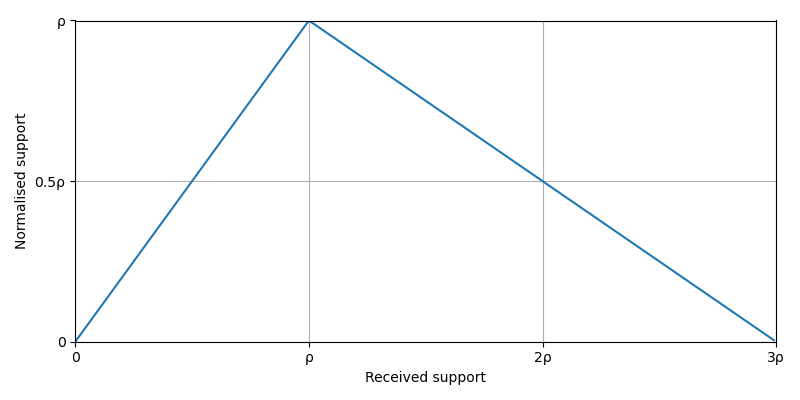
\includegraphics[width=0.99\textwidth]{norm_support}
    \caption[Inhibition for too many activated cells]{The visualisation of formula \eqref{norm_2}. The x-axis shows the received support, and the y-axis shows the support after normalisation: As soon as the received support is bigger than $\rho$, it is reduced with a slope of $-0.5$.}
    \figlbl{norm_support}
\end{figure}
This function is visualised in \figref{norm_support}. No normalisation is applied if a cell's activation is below $\rho$. However, if the activation is above $\rho$, the cell's lateral support strength is decreased with a slope of $-0.5$. Experimental findings suggest that this upper support limit helps overcome varying support strengths during training.



\subsection{Alternative Cells}\seclbl{framework_alt_cells}
As described in \secref{neuroscience_findings_alt_cells}, alternative cells and pathways are necessary to deal with different patterns that activate similar feature cells.
``Alternative'' in this context means that only one cell among the alternatives is active, i.e. these cells are mutually exclusive.
At the beginning of training, alternative cells are copies of an initial cell.
However, after training, these cells contribute to different patterns and have different behaviour.

Alternative cells can be implemented by adding additional (alternative) output channels.
The duplication factor $\kappa$ defines how many alternative channels should be added.
Thus, the weight $\boldsymbol{W}$ with alternative cells is of shape $\left[(\kappa \cdot C_{\text{out}}) \times C_{\text{in}} \times (2n+1) \times (2n+1)\right]$.

\begin{figure}[h]
    \centering
    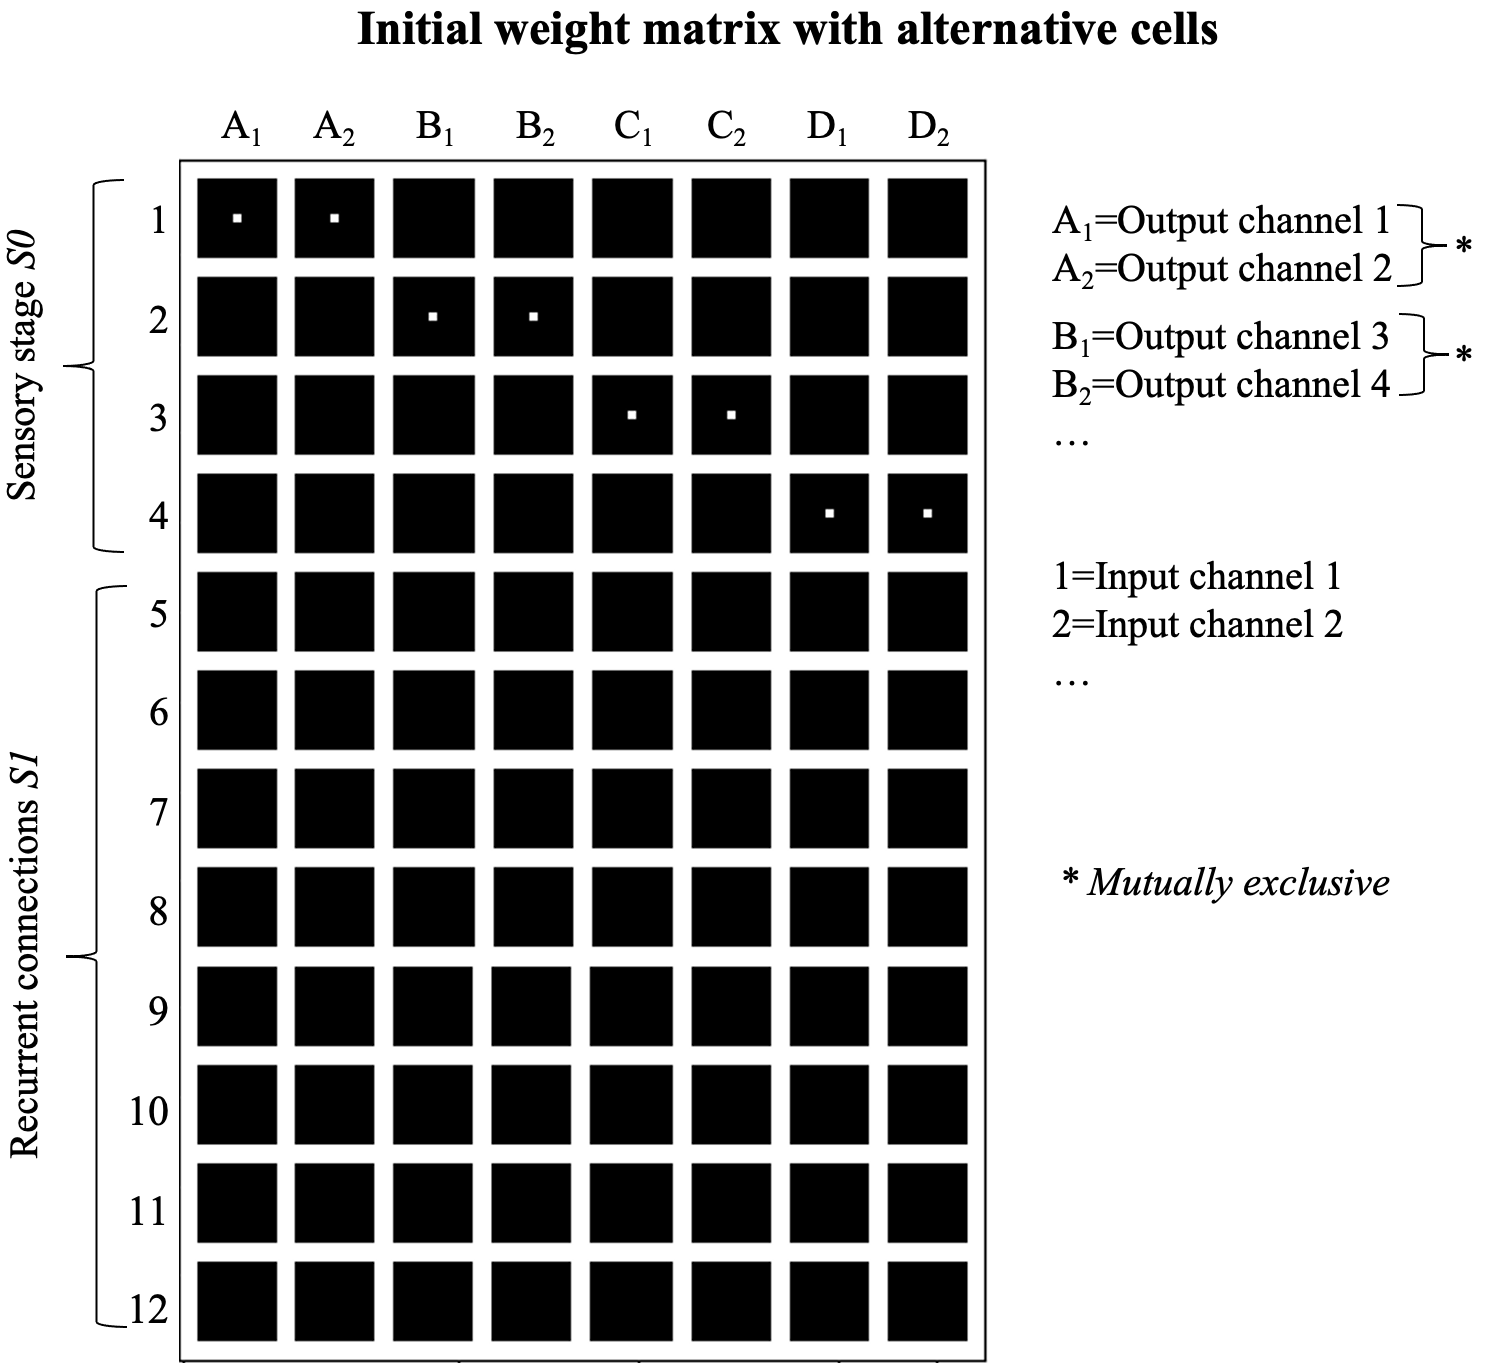
\includegraphics[width=0.99\textwidth]{lateral_init_weights_alt}
    \caption[Initialisation of the lateral weight matrix with alternative cells]{Initialisation of the lateral weight matrix with alternative cells. The initialisation is similar to the one shown in \figref{lateral_init_weights}, except each channel is duplicated $\kappa=2$ times.}
    \figlbl{lateral_init_weights_alt}
\end{figure}

In \figref{lateral_init_weights_alt}, it is visualised how the weight $\boldsymbol{W}$ with a duplication factor of $\kappa=2$ are initialised.
In that case, $\kappa=2$ output channels are mutually exclusive, leading to activation in only one of these channels.
Implementing mutually exclusive cells requires competition between alternative cells \sidecite{von_der_malsburg_neural_1987} so that only the most suitable cell can remain active if multiple exclusive cells are active.
For example, such competition can be implemented by comparing how well a specific activation pattern fits the already learned lateral support \cite{vogels_inhibitory_2011, joshi_rules_2009, teichmann_intrinsic_2015}.
Another option is implementing inhibition between the competing channels so that the dominant channel turns off the other channels.


\subsection{Measuring Support Quality}\seclbl{S1_goodness}
After learning net fragments, it is crucial to evaluate their quality.
A simple approach is to measure the support needed to remain active and the average support active and inactive cells receive.
At the beginning of training, self-support is used, and therefore, the average support of active cells is $1$, and the average support of inactive cells is $0$.
However, during training, lateral connections are learned that support cells to remain active.
This leads to higher activation in general, which, in turn, increases the threshold to remain active.
Thus, the average activation of the cell increases as well as the threshold to remain active.
These statistics can be measured over the training process to evaluate the quality of the net fragments.

As a second metric, we can measure the robustness against noise.
Net fragments should only support cells that are activated by a learned pattern. Thus, cells activated by noise should not receive enough support and be turned off after a few cycles.
Therefore, as a second metric, we can add noise to the input image and measure how many cells in the sensory system are activated due to the noise and what ratio of them remains active after applying lateral connections.


\section{Prototype Stage \emph{S2}}\seclbl{framework_s2}
In stage \emph{S2}, the net fragments are mapped to idealised reference objects.
This mapping is implemented by projection fibres \cite{tanigawa_organization_2005, greig_molecular_2013}, which are grouped into maplets \sidecite{zhu_maplets_2004}.
As soon as a control unit of a maplet detects a strong correlation between the neurons it connects in \emph{S1} and \emph{S2}, it initialises the mapping by turning on its fibres.

This mapping from fragments to reference representations seems to be one of the core algorithms of the biological visual system as it can solve the binding problem \sidecite{revonsuo_binding_1999, feldman_neural_2013}, i.e. answers the questions of how visually perceived objects are bound together based on their properties such as shape, texture, colour, contour, or motion.

Implementing such a mapping poses various challenges.
In the following, some simplifications are assumed that are ignored in the proposed framework and have to be solved in future work.
\begin{itemize}
    \item \textbf{Storing object prototypes in \emph{S2}}: It is assumed that the reference representations are already stored in \emph{S2}. Consequently, the mapping process is reduced to finding the most suitable projection, disregarding that the object prototype might not be stored yet. Nevertheless, it would be desirable that the network can, for example, when encountering high uncertainty, autonomously recognise the absence of a proper object prototype and create one.
    \item \textbf{Enhancing object prototypes in \emph{S2}}: It is assumed that the object prototypes are idealised, can remain static, and do not require further updates. 
    Findings from psychology suggest that our brain is highly structured and might contain such prototypes from birth \sidecite{simion_face_2015}. However, these prototypes are also known to be optimised with increasing experience over time \cite{simion_face_2015}.
    Moreover, updating prototypes is important when novel prototypes are stored, as an optimised form of such a reference object typically cannot be derived from a single sample.
    \item \textbf{Object-centered input}: The input images are assumed to contain exactly one object rather than complex scenes containing multiple objects. This allows to map a part of an image, i.e. the region where the object is located, to exactly one object reference frame. In real-world scenarios, visual scenes often comprise multiple objects, requiring the model to map a single input to multiple prototypes. Consequently, an attention mechanism becomes essential to identify object boundaries before comparing them to suitable references.
    \item \textbf{Pre-defined projection fibres}: It is assumed that the projection fibres already exist from the beginning and remain unchanged throughout the learning process. Thus, the learning process focuses on the activation of control units. This assumption requires pre-defining many fibres, some of which may be unnecessary, making the system less efficient. Dynamically growing or pruning fibres could make the system more efficient and robust.
\end{itemize}

\subsection{Correspondence-Mapping}
\begin{figure}[h]
    \centering
    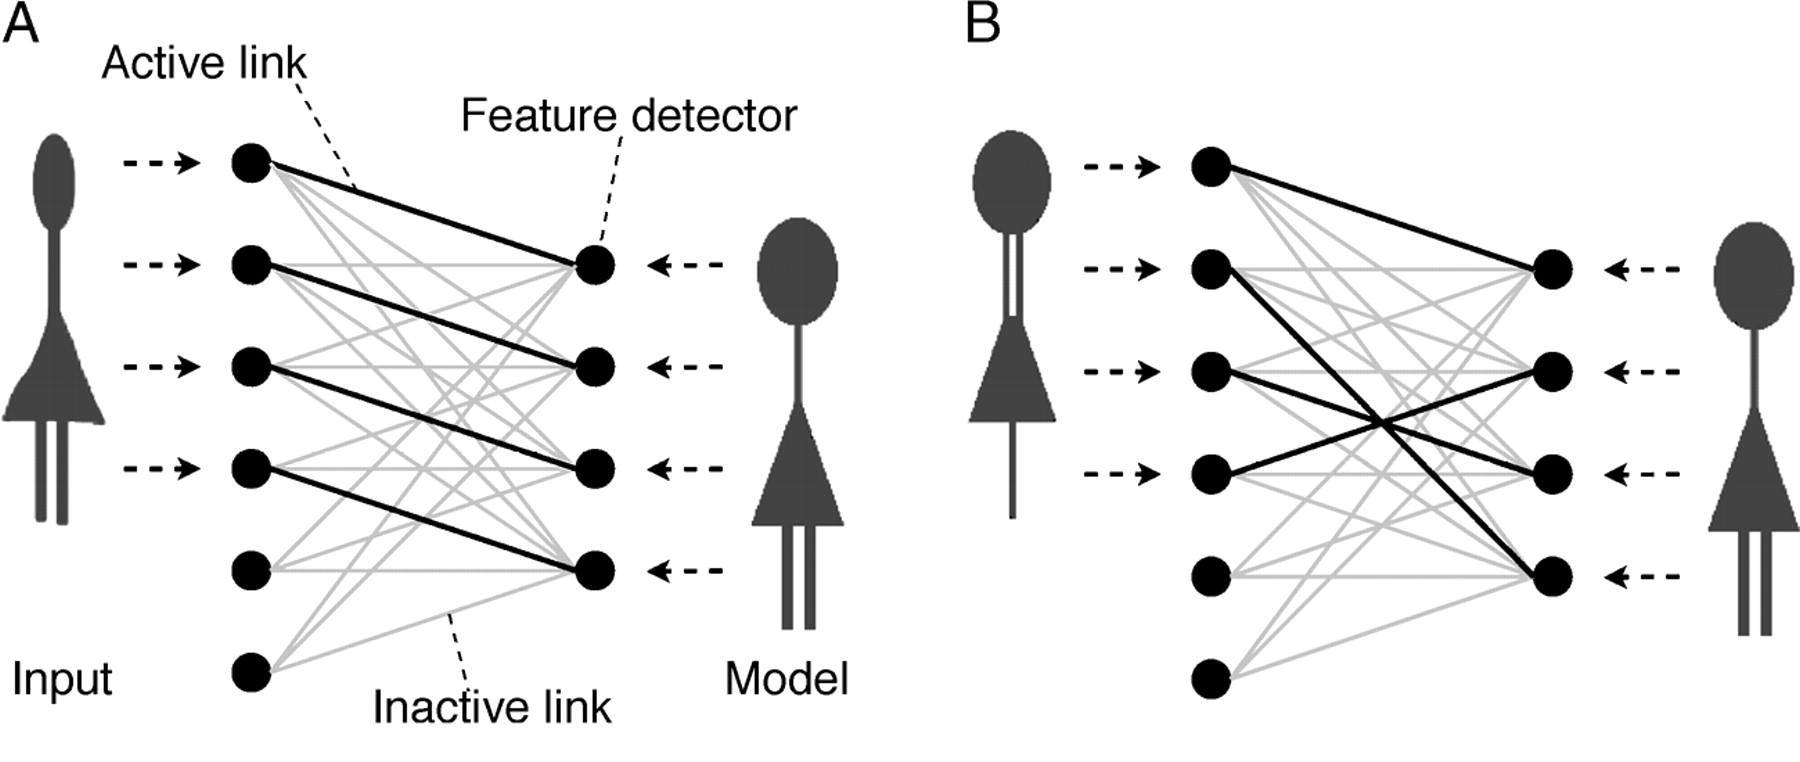
\includegraphics[width=0.99\textwidth]{correspondence_recognition}
    \caption[The visual correspondence problem]{Visualisation of the correspondence problem: Corresponding points between an input and a model must be linked. All potential correspondences are visualised as grey lines, while the correct correspondences are shown as black lines. Example $\boldsymbol{A}$ shows a correct correspondence, while example $\boldsymbol{B}$ visualises a wrong correspondence, although similar features are connected. The image is from \cite{wolfrum_recurrent_2008}.}
    \figlbl{correspondence_recognition}
\end{figure}

So far, the problem is described as mapping entire net fragments to object prototypes.
However, this is a somewhat simplified view, as many similar objects differ slightly.
Therefore, one cannot just compare objects but rather multiple features that define an object.
This problem of mapping features extracted from an input image to features from a reference object is known as the correspondence problem.
\sideciteay{wolfrum_recurrent_2008} motivate the correspondence problem based on \figref{correspondence_recognition}. This figure depicts two stick figures where the input's features, such as the head or neck, must be linked to the corresponding model's features.
There exist various mappings, symbolised as grey lines.
The correspondence problem is to find a subset of these links that are the correct correspondences (visualised as black lines in example $\boldsymbol{A}$). 

Unfortunately, it is not sufficient to calculate the similarity between features as illustrated in 
\figref{correspondence_recognition} example $\boldsymbol{B}$. Different images of the same object can vary significantly, resulting in a high degree of similarity between non-corresponding features \sidecite{wiskott_role_1999}. The reason is that not only the features define an object but also their spatial arrangement. Therefore, correspondence-based systems must take both into account.

\begin{figure}[h]
    \centering
    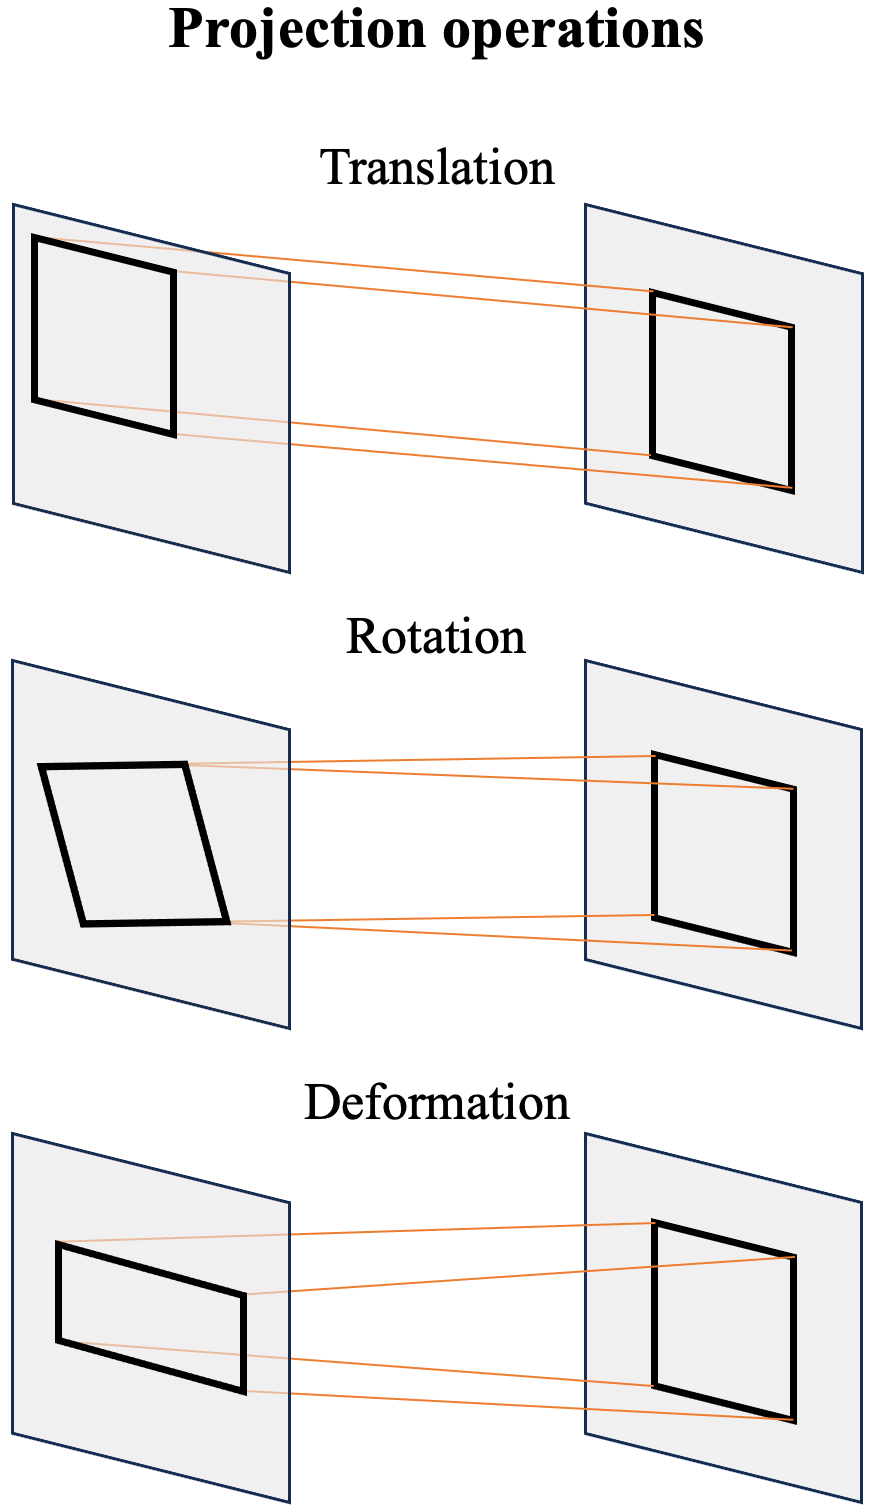
\includegraphics[width=0.5\textwidth]{projection_operations}
    \caption[Different projection operation]{Different projection operations that must be implemented with projection fibres. Projection fibres should make the mapping process invariant to translation, rotation, and deformation.}
    \figlbl{projection_operations}
\end{figure}
In \figref{projection_operations}, the operations needed to deal with different spatial arrangements are visualised.
Projection fibres must be invariant to translation, rotation, and deformation. Such transformation can occur globally, as depicted in \figref{projection_operations}, and locally.
In \secref{framework_s2_sim}, it is described how the similarity between local areas connected by a projection fibre can be measured. This statistic is needed to decide whether a control unit should switch on. Subsequently, in \secref{framework_s2_mapping}, it is described how the projection fibres can be wired.

\subsection{Measuring Similarity}\seclbl{framework_s2_sim}
Correspondence-based mapping requires measuring feature similarity.
Since binary neurons are used, similarity can be calculated by comparing the neurons' activity. They are similar if both neurons are on or off; if one neuron is on while the other is not, they are dissimilar.
However, multiple neurons exist at the same spatial location, representing various features.
The mapping process compares how similar the spatial locations between a net fragment and a corresponding location of the reference object are.
Therefore, all neurons at the same location are compared.

Both the net fragments in \emph{S1} and the prototypes in \emph{S2} are of shape $[C_{\text{out}} \times W \times H]$. Thus, per spatial location $(x,y)$ (where $x \in \{0, ..., W\}$ and $y \in \{0, ..., H\}$), exists a one-dimensional feature vector of length $C_{\text{out}}$. This vector is denoted as $\boldsymbol{a}_{S1,(x,y)}$ for \emph{S1} and $\boldsymbol{a}_{S2,(x,y)}$ for \emph{S2}.
These two vectors can be compared using the Jaccard similarity $J$, which is defined as:
%
\begin{align}\eqlbl{jaccard}
	J_{x,y} = J(\boldsymbol{a}_{S1,(x,y)}, \boldsymbol{a}_{S2,(x,y)}) = \frac{|\boldsymbol{a}_{S1,(x,y)} \cap \boldsymbol{a}_{S2,(x,y)}|}{|\boldsymbol{a}_{S1,(x,y)} \cup \boldsymbol{a}_{S2,(x,y)}|}
\end{align}
%
The term $|\boldsymbol{a}_{S1,(x,y)} \cap \boldsymbol{a}_{S2,(x,y)}|$ describes the number of corresponding cells that are activated in both \emph{S1} and \emph{S2}, while the second term $|\boldsymbol{a}_{S1,(x,y)} \cup \boldsymbol{a}_{S2,(x,y)}|$ is the number of cells that are activated in either \emph{S1} or \emph{S2}. Features that are deactivated in \emph{S1} and \emph{S2} are not taken into account.
The Jaccard similarity $J$ is in the range of $(0, ..., 1)$, where $1$ is the highest possible similarity.

As motivated in \figref{correspondence_recognition} example $\boldsymbol{B}$, having a high similarity between two feature vectors is not enough to describe the quality of a projection, as also the spatial arrangement must be considered.
Therefore, not only the similarity between two spatial locations $(x,y)$ is compared but all neurons in a local neighbourhood.
\begin{figure}[h]
    \centering
    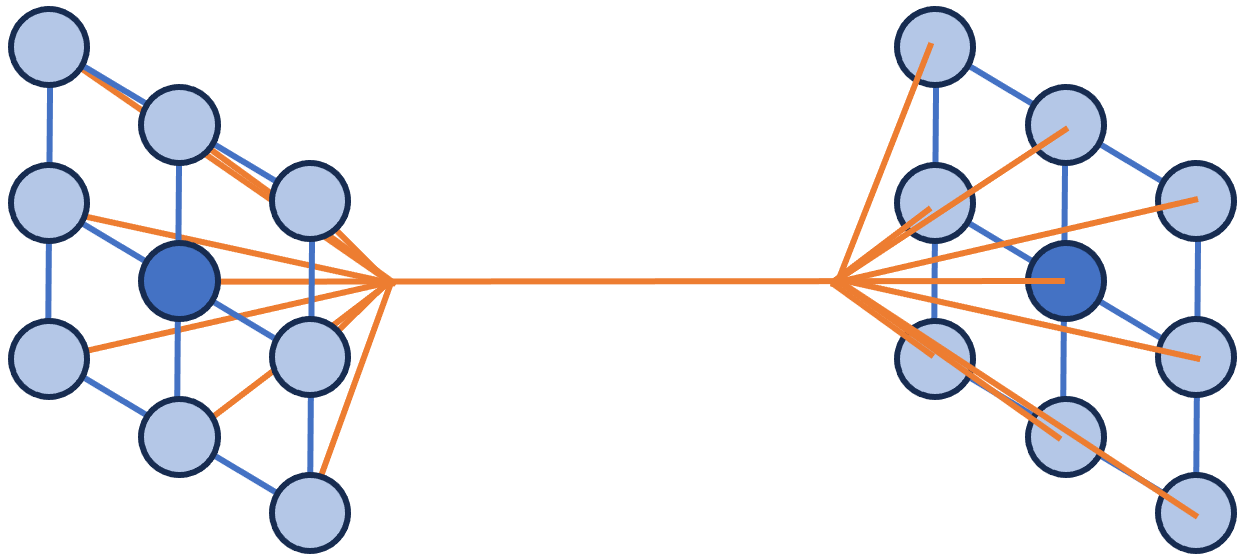
\includegraphics[width=0.7\textwidth]{jaccard_similarity}
    \caption[Similarity between two vectors and their spatial neighbours]{The Jaccard similarity between two vectors (coloured in dark blue) and their spatial neighbours (coloured in light blue).}
    \figlbl{jaccard_similarity}
\end{figure}
Such a comparison is visualised in \figref{jaccard_similarity}:
The similarity between the two vectors (depicted as dark blue circles) also depends on their local neighbours (light blue circles).
The size of the local neighbourhoods is defined as $n_J$, and the local neighbourhoods as $\boldsymbol{A}_{S1,(x,y)} = ( \boldsymbol{a}_{S1,(x-n_J,y-n_J)}, ..., \boldsymbol{a}_{S1,(x+n_J,y+n_J)} )$ and $\boldsymbol{A}_{S2,(x,y)} = ( \boldsymbol{a}_{S2,(x-n_J,y-n_J)}, ..., \boldsymbol{a}_{S2,(x+n_J,y+n_J)} )$, respectively.
The Jaccard similarity between two vectors that consider the local neighbourhood is thus defined as:
%
\begin{align}\eqlbl{jaccard2}
	J_{x,y} = J \left( \boldsymbol{A}_{S1,(x,y)}, \boldsymbol{A}_{S2,(x,y)} \right)
\end{align}
%
Considering a local neighbourhood can be likened to having local support, as is the case for net fragments. Multiple cells must support the mapping to be activated by the corresponding control unit. For example, the similarity between two dissimilar vectors can still be high if their context is similar, which helps deal with noise in the data.
On the other hand, the similarity between two identical vectors is low if their context is dissimilar and therefore does not match.
Such local support thus increases robustness and provides higher similarity for spatially correctly arranged features.


\subsection{Mapping Process}\seclbl{framework_s2_mapping}
In the previous section, it is discussed how the similarity between activity patterns of neurons connected by projection fibres can be calculated.
In the following, it is described how projection fibres can be wired.

\begin{figure}[h]
    \centering
    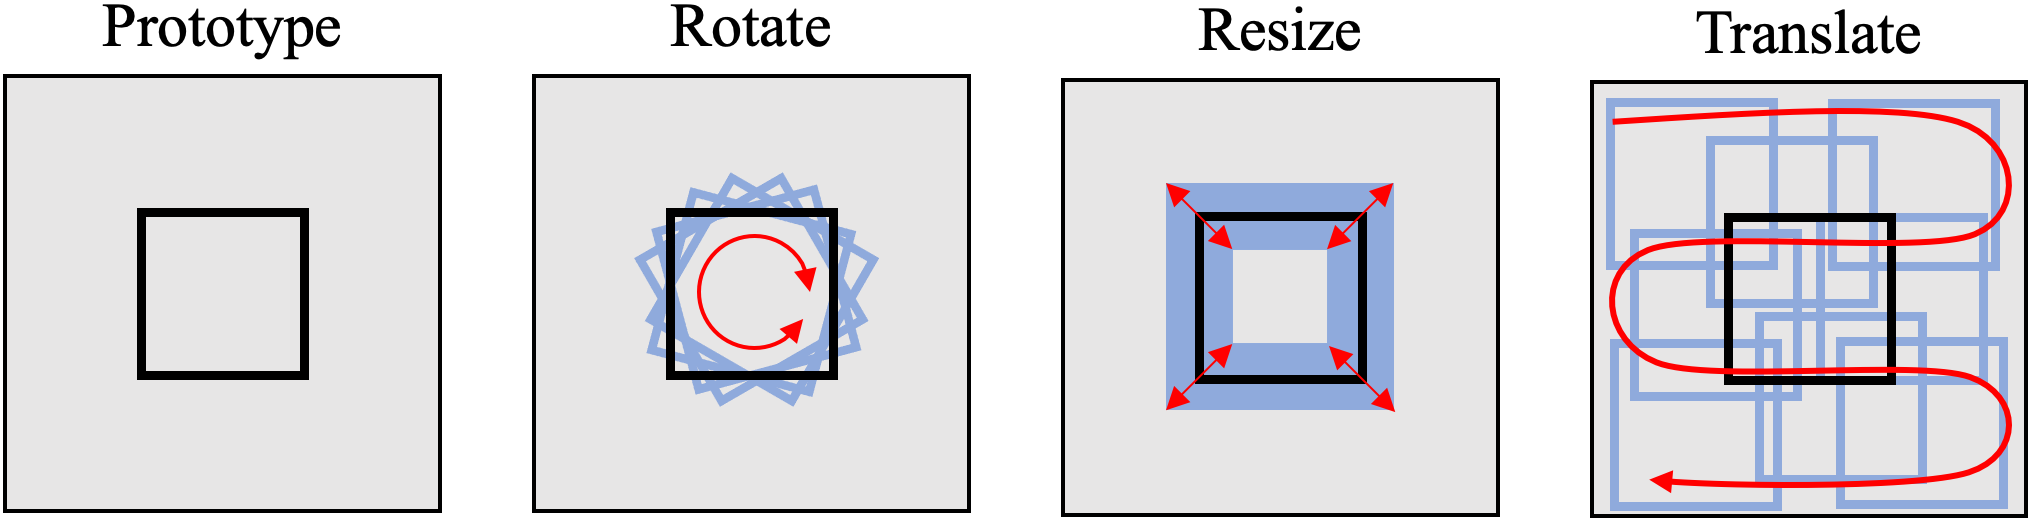
\includegraphics[width=0.99\textwidth]{prototype_operations}
    \caption[Operations applied to a prototype]{Different operations applied to a prototype.}
    \figlbl{prototype_operations}
\end{figure}
A straightforward approach is to apply different operations such as translation, rotation, and deformation to a reference frame as shown in \figref{prototype_operations}. These operations can be used individually or in combination, resulting in multiple augmented prototype versions.
Thereby, the shift of each neuron is tracked, and a projection fibre is used to map a neuron from the prototype to the corresponding neuron in the augmented version.

However, such an object-dependent mapping would not scale as each object requires a multitude of fibres.
Instead, the mapping must be object-independent and focus on local features.
In this context, ``object-independent'' still means that the feature similarity has to be calculated per object but that not each different object requires a unique set of projection fibres.
Shifter circuits \sidecite{anderson_shifter_1987, olshausen_neurobiological_1993} are a kind of hierarchical mapping that implement such an object-independent mapping focusing on local features.
Shifter circuits define different hierarchical levels, whereby each level is responsible for a specific operation, such as a rotation, shift, or translation.
During the fast processing loop when the input image is static, very fast Hebbian plasticity \sidecite{hebb_organization_1949} can be used to create a topographical projection, i.e. to connect neighbouring cells in \emph{S1} with neighbouring cells in \emph{S2} as shown by \sideciteay{fernandes_self-organization_2015}.
Furthermore, \citeay{fernandes_self-organization_2015} also demonstrates that the medium processing loop providing different image views can be leveraged to teach the model what the same object from different viewpoints looks like.
This helps to improve the mapping processing and the prototypes.

Each projection fibre calculates the similarity between the neurons it connects when processing an image.
Afterwards, the average similarity is calculated per maplet, and this similarity is used as the activation probability of a Bernoulli neuron that can turn on the corresponding control unit.
Similar to \emph{S1}, this leads to many activations at the beginning and inhibition is used to turn some of the maplets off.
Maplets support each other locally and can only remain active if neighbouring features in \emph{S1} remain neighbouring features in \emph{S2}.
Thus, the better a set of maplets can map a prototype to an object reference, the higher its probability of remaining active.
For more details on the implementation, please refer to the work by \citeay{anderson_shifter_1987}, \citeay{olshausen_neurobiological_1993}, and \citeay{fernandes_self-organization_2015}.


\subsection{Feedback to \emph{S1}}
\emph{S2} serves two purposes: It not only maps an input to a reference frame to obtain a transformation-invariant representation but also provides feedback to \emph{S1} by mapping the reference object back to \emph{S1}.
To provide feedback, the most plausible prototype is selected.
As described in \secref{framework_s1}, this prototype from \emph{S2} can overwrite the representations in \emph{S1} and is thus incorporated into the learning process in \emph{S1}.

The representations in \emph{S1} and \emph{S2} might slightly vary as the net fragments in \emph{S1} represent a particular instance of an object. In contrast, \emph{S2} represents a generalised (optimised) version of the same object.
However, these representations should still be similar (otherwise, a proper prototype in \emph{S2} is missing).
Therefore, \emph{S1} receives an optimised version of the net fragments as input. This can be considered a bias towards a better representation.
By applying Hebbian updates between the input in \emph{S1} and the prototypes from \emph{S2}, \emph{S1} learns to convert its features to an optimised version.
Thus, the feedback from \emph{S2} provides additional support in \emph{S1} and can help to build better representations and fragments.


\subsubsection{Measuring \emph{S2} Quality}\seclbl{S2_goodness}
\emph{S2} can be considered an associative memory, mapping net fragments to the most suitable reference frame.
A strength of such a system is that it is highly robust and can deal well with noisy data or occluded objects \sidecite{ramsauer_hopfield_2021}.
Therefore, \emph{S2} can be evaluated by occluding data and letting it reconstruct it as it is done for many deep learning systems \sidecite{han_image-based_2021, qu_transmef_2022}. 

Furthermore, \emph{S2} maps net fragments to object prototypes. Thus, another way to evaluate the quality of \emph{S2} is to measure if the input is mapped to the corresponding object prototype.
The mapping accuracy can be measured on an object or feature level with typical classification metrics \sidecite{schmarje_survey_2021} such as accuracy or F1-score.

Please note that \emph{S2} highly depends on \emph{S1}. To evaluate the performance \emph{S2} independently, it has to be encapsulated from \emph{S1}.
This can be achieved using strongly augmented reference objects from \emph{S2} as input instead of actual net fragments from \emph{S1}.
